% !TeX program = xelatex
% !TeX encoding = UTF-8
% !TeX spellcheck = en_US
\documentclass[UTF8,a4paper,zihao=-4,fontset=fandol]{ctexart}
% !TeX root = main.tex
% 中文字体随 TeX Live 提供，可随工程迁移，不依赖 Windows 专用字体。
\usepackage[left=25mm,right=25mm,top=25mm,bottom=25mm]{geometry}
\setmainfont{texgyretermes-regular.otf}[
  BoldFont=texgyretermes-bold.otf,
  ItalicFont=texgyretermes-italic.otf,
  BoldItalicFont=texgyretermes-bolditalic.otf]
\usepackage{amsmath,amssymb}
\usepackage{graphicx}
\usepackage{float}
\usepackage{placeins}
\usepackage[font=small,labelfont=bf,labelsep=quad,
            justification=justified,singlelinecheck=false]{caption}
\usepackage{booktabs}
\usepackage{enumitem}
\usepackage[noadjust,nocompress]{cite}
% IEEE inline numeric citations; stable first-citation numbering.
\renewcommand{\citepunct}{], [}
\renewcommand{\refname}{References}
\usepackage[unicode,hidelinks]{hyperref}
\hypersetup{pdftitle={RBSRN}}
\ctexset{
  section={format=\Large\bfseries,number=\arabic{section},
           beforeskip=1.2ex plus 0.5ex,afterskip=0.8ex plus 0.2ex},
  subsection={format=\large\bfseries,beforeskip=1ex plus 0.3ex,
              afterskip=0.6ex plus 0.2ex}
}
\linespread{1.2}
\setlength{\parindent}{2em}
\setlength{\parskip}{0pt}
\setlength{\emergencystretch}{2em}
\setlist[enumerate]{leftmargin=2em,label=\arabic*.,itemsep=0.25em,topsep=0.4em}
\providecommand{\tightlist}{\setlength{\itemsep}{0pt}\setlength{\parskip}{0pt}}
\allowdisplaybreaks[1]
\clubpenalty=10000
\widowpenalty=10000
\raggedbottom
\pagestyle{plain}

% Compact, readable float placement; retain the original font size and margins.
\DeclareCaptionFont{compact}{\linespread{1.05}\selectfont}
\captionsetup{font={small,compact},skip=5pt}
\setlength{\textfloatsep}{11pt plus 2pt minus 2pt}
\setlength{\floatsep}{9pt plus 2pt minus 2pt}
\setlength{\intextsep}{10pt plus 2pt minus 2pt}
\renewcommand{\topfraction}{0.95}
\renewcommand{\bottomfraction}{0.90}
\renewcommand{\textfraction}{0.05}
\renewcommand{\floatpagefraction}{0.75}
\setcounter{topnumber}{4}
\setcounter{bottomnumber}{3}
\setcounter{totalnumber}{6}
\makeatletter
\setlength{\@fptop}{0pt}
\setlength{\@fpsep}{10pt}
\setlength{\@fpbot}{0pt plus 1fil}
\makeatother
\AtBeginDocument{%
  \setlength{\abovedisplayskip}{8pt plus 2pt minus 2pt}%
  \setlength{\belowdisplayskip}{8pt plus 2pt minus 2pt}%
  \setlength{\abovedisplayshortskip}{3pt plus 1pt minus 1pt}%
  \setlength{\belowdisplayshortskip}{6pt plus 1pt minus 1pt}}

% Keep each figure/table inside its owning section, subsection and subsubsection.
\AddToHook{cmd/section/before}{\FloatBarrier}
\AddToHook{cmd/subsection/before}{\FloatBarrier}
\AddToHook{cmd/subsubsection/before}{\FloatBarrier}

% Local revision markup is visible only in main-revision-marked.tex.
\providecommand{\revised}[1]{#1}

% Final inference revision; earlier revision marks remain black.
\providecommand{\infrevised}[1]{#1}

% Original supplementary Fig. S1 promoted to main-text Fig. 7.
\providecommand{\soneupdated}[1]{#1}

% Hyperparameter prose and evidence-placement revision (2026-11-04).
\providecommand{\hpupdated}[1]{#1}

% Reference-wording revision (2026-11-04).
\providecommand{\refupdated}[1]{#1}

% Caption, note and full-reference audit (2026-11-04).
\providecommand{\editorialupdated}[1]{#1}

\providecommand{\ablationpolished}[1]{#1}

\providecommand{\spatialpolished}[1]{#1}

\providecommand{\scenariopolished}[1]{#1}

% Baseline and metric section restructuring (2026-11-05).
\providecommand{\metricrevised}[1]{#1}

% PDFormer corrected results (2026-11-06).
\providecommand{\pdformerupdated}[1]{#1}

% Shanghai epoch115 update (2026-11-06)
\providecommand{\shanghaiupdated}[1]{#1}

% First-citation order and source-grounded reference revision (2026-11-06).
\providecommand{\citationupdated}[1]{#1}
\providecommand{\citationbibliographystyle}{}

% Merged discussion and conclusion revision (2026-11-06).
\providecommand{\conclusionrevisionstyle}{}

% !TeX root = main.tex
% English title, keywords, and PDF metadata; author details remain to be supplied.
\newcommand{\papertitle}{RBSRN: Role-Aware and Background-Conditioned Residual Refinement for Multi-Step Regional Traffic Flow Forecasting}
\newcommand{\paperkeywords}{regional traffic flow forecasting; multi-step forecasting; spatiotemporal residual learning; role-aware gating; background-conditioned historical message selection}
\title{\papertitle}
\author{}
\date{}
\hypersetup{pdftitle={RBSRN: Role-Aware and Background-Conditioned Residual Refinement for Multi-Step Regional Traffic Flow Forecasting},
  pdfsubject={Multi-step regional traffic flow forecasting},
  pdfkeywords={regional traffic flow forecasting; multi-step forecasting; spatiotemporal residual learning; role-aware gating; background-conditioned historical message selection}}
% Compact title block for the current ctexart working manuscript.
% When author details become available, fill \author in this file.
\makeatletter
\renewcommand{\@maketitle}{%
  \begin{center}
    {\fontsize{17}{20}\selectfont\bfseries\@title\par}
    \ifx\@author\@empty\else
      \vspace{0.7em}{\normalsize\@author\par}
    \fi
  \end{center}\vspace{0.2em}}
\makeatother

\newcommand{\frontmatterrevisionstyle}{}

\begin{document}
% !TeX root = ../main.tex
% !TeX encoding = UTF-8
% English title, abstract, and keywords; single-paragraph abstract.
\begingroup
\maketitle
\frontmatterrevisionstyle
\begin{center}
  \normalsize\bfseries Abstract
\end{center}
{\small\setlength{\parindent}{0pt}
Short-term, multi-step regional traffic flow forecasting uses recent observations to estimate future inflow and outflow for traffic dispatch. When local flow deviates from routine patterns, self-evolution and cross-region historical information play different correction roles. Historical correlations alone do not establish their relevance in the current traffic context or at different forecast horizons. We propose the Role-aware and Background-conditioned Spatiotemporal Residual Network (RBSRN), which refines a base prediction through two parallel branches. The first fuses residual corrections from self-evolution and directed time-lagged experts according to the current state. The second performs Background-conditioned Cross-region Message Selection (BCMS), jointly selecting neighbor--lag--scale messages for each forecast step using source and target traffic backgrounds. We evaluated RBSRN against 13 baseline methods on four inflow and outflow forecasting tasks in Chengdu and Shanghai. RBSRN achieved the lowest mean absolute error (MAE) averaged over 12 forecast steps under positive-target evaluation. Its MAE was 0.43\%--2.00\% lower than that of the strongest baseline method for each task. Fixed-model residual-removal diagnostics showed that, among high-deviation samples, the MAE benefit of self-evolution correction at the 30-minute horizon was 1.15--2.82 times as large for rapidly changing histories as for slowly changing histories. BCMS, in turn, provided its largest mean benefit in the group with the lowest history-derived background-discrepancy proxy values at all 12 forecast steps. Together, these results support prediction correction conditioned on traffic state and background.
\par\vspace{0.8em}
\noindent\textbf{Keywords: }\paperkeywords
\par}
\endgroup
\vspace{1em}


\captionsetup[figure]{name=Figure}
% !TeX root = ../main.tex
% !TeX encoding = UTF-8
% !TeX spellcheck = none

\section{Introduction}\label{sec:introduction}

Anticipating travel demand across urban regions supports fleet dispatch and the allocation of transport resources~\cite{ref44}. Regional inflow and outflow describe trips arriving in and departing from each region within a given interval~\cite{ref36}; their variation determines where demand concentrates, how large it becomes, and how long it persists. Dispatch decisions require forecasts of successive increases, decreases, and spatial shifts in demand to guide vehicle deployment and regional service provision~\cite{ref27,ref43}. Short-term multi-step traffic flow forecasting therefore jointly estimates regional inflow and outflow at successive future time steps from recent observations, supporting dispatch decisions over the next 5--60 minutes. \citationupdated{Traffic event information has been used to supplement historical traffic observations and improve short-term flow forecasting~\cite{ref42}}. Improving multi-step regional forecasting requires models to capture routine spatiotemporal patterns while responding to local changes in demand.

Traffic flow forecasting has progressed through advances in spatial dependency learning, temporal pattern representation, and multiscale dynamics modeling. For regional flow forecasting, ST-ResNet uses residual convolutions to jointly model temporal closeness, periodicity, and trends. In its single-step TaxiBJ experiment at a 30-minute resolution, the best configuration reduced RMSE from DeepST's 18.18 to 16.69, a relative decrease of approximately 8.2\%~\cite{ref14}. Spatiotemporal graph networks combine inter-node relations with temporal encoding, learning spatial dependencies through diffusion convolution, graph convolution, and adaptive adjacency matrices~\cite{ref01,ref02,ref03}. STWave and TEDDCF use frequency decomposition and two-branch encoding to represent low-frequency trends and high-frequency dynamics separately~\cite{ref11,ref18}. \citationupdated{ST-GDN further combines local geographic dependencies, global regional associations, and multiscale temporal attention to organize historical information~\cite{ref41}}. These studies broaden the historical information available to forecasting models, drawing on node trajectories, cross-region relations, and temporal patterns at different scales. When local flow deviates from routine patterns, however, the relevance of this historical evidence needs to be reassessed in light of the current state. Determining its relevance at different forecast horizons and translating it into effective prediction corrections remain important questions for short-term multi-step forecasting.

These issues concern both the sources of evidence and the conditions under which historical messages are useful. A node's own history directly records the continuation and turning points of its local state, whereas observations from other regions provide cross-region references through directed time-lagged associations~\cite{ref47}. These sources differ in their spatial origins, temporal alignment, and correction roles. Even for the same neighbor, historical messages correspond to different lag positions and scales of variation; \citationupdated{their relevance must be assessed using the source and target traffic backgrounds and the forecast horizon}. \editorialupdated{Figure~\ref{fig:intro-case} illustrates these differences using outflow from grid cell 601 in Chengdu in November 2016:} for two recent traffic states, the historical correlations between the target and a lag-aligned neighboring region were 0.859 and 0.907, respectively, whereas the mean absolute differences between their observed trajectories over the subsequent 30--60 minutes were 0.5 and 6.0 counts per 15 min. Both states exhibited strong historical associations but differed in how far their subsequent trajectories diverged. This observation focuses attention on the conditions under which historical information remains useful. Self-evolution and cross-region time-lagged evidence need distinct roles in correcting the base prediction, while historical messages need to be selected for each future forecast step according to the current background.

Existing approaches address heterogeneous dynamics and cross-region information through signal disentanglement, expert routing, and delay awareness. D2STGNN separates diffusion and inherent signals through gating and residual decomposition, then models them with different modules~\cite{ref25}. TESTAM uses temporal, static-graph, and dynamic-graph experts, adapting to different traffic conditions through routing~\cite{ref26}. PDFormer combines dynamic spatial attention with delay-aware feature transformations to address temporal misalignment in cross-region information~\cite{ref10}. These studies provide a basis for distinguishing sources of dynamics and establishing spatiotemporal associations, making the organization of prediction evidence more explicit. For multi-step regional forecasting under local deviations, linking such differentiated modeling to correction benefits requires understanding when self-evolution and directed time-lagged information improve the base prediction, and how the benefits of cross-region historical messages vary with source--target background discrepancy and forecast horizon.

\begin{figure}[!t]
	\centering
	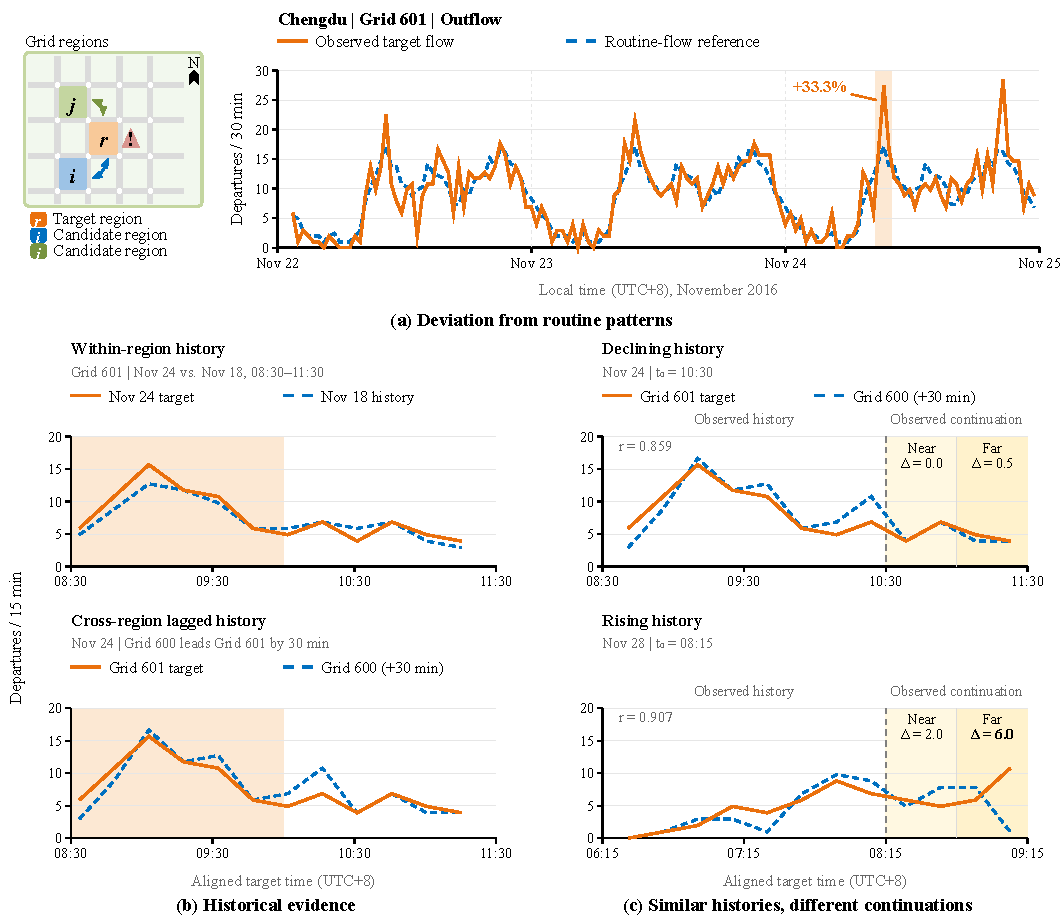
\includegraphics[width=\linewidth]{figures/introduction-case.pdf}
	\caption{\editorialupdated{Observed deviations from routine flow patterns and historical references. (a) Routine-flow reference and observed flow. (b) Within-region and cross-region historical evidence. (c) Divergent subsequent trajectories following similar histories.}}
	\label{fig:intro-case}
\end{figure}

We introduce the Role-aware and Background-conditioned Spatiotemporal Residual Network (RBSRN) to organize correction evidence and select historical messages when local flow deviates from routine patterns. RBSRN refines a base prediction through adaptive fusion of heterogeneous experts and background-conditioned selection of historical messages. Shared dual-frequency spatiotemporal encoding first extracts low- and high-frequency representations and generates the base prediction. The State-Evidence Expert Residual Refinement Module (SERR) assigns distinct roles to self-evolution and directed time-lagged experts and allocates their correction contributions according to the current state. Background-conditioned Cross-region Message Selection (BCMS) uses the low-frequency source and target traffic backgrounds to jointly select high-frequency historical messages for each forecast step. Both modules read the shared representations in parallel, and their corrections are added at the prediction stage to jointly forecast regional inflow and outflow over multiple future steps.

The main contributions are as follows:

\begin{enumerate}
	\def\labelenumi{\arabic{enumi}.}
	\item
	To account for heterogeneous prediction evidence and allocate its contributions under deviations from routine patterns, we introduce SERR. Its state-conditioned gate combines residual corrections from self-evolution and directed time-lagged experts to refine the base prediction according to the current state. \revised{Ablation experiments on Chengdu showed that removing either expert increased both MAE and RMSE for inflow and outflow.}
	\item
	To account for changes in the relevance of cross-region historical evidence across traffic backgrounds and forecast horizons, we introduce BCMS. It jointly selects neighbor--lag--scale messages for each forecast step, providing background-conditioned and horizon-specific residual corrections to the base prediction. Fixed-model residual-removal diagnostics in both cities showed larger average MAE benefits from these corrections when the history-derived proxy for background discrepancy between the target and candidate source regions was smaller.
	\item
	We systematically evaluated RBSRN's forecasting performance and residual refinement on the Chengdu and Shanghai datasets. In the overall comparison with 13 representative baseline methods, RBSRN achieved the lowest AVG12 MAE on all four city--channel forecasting tasks, reducing MAE by \shanghaiupdated{0.43\%}--2.00\% relative to each task's strongest baseline method. \shanghaiupdated{It also achieved the lowest AVG12 RMSE on all four tasks}.
\end{enumerate}

% !TeX root = ../main.tex
% !TeX encoding = UTF-8
% !TeX spellcheck = none

% Reference identities and placements retained from the verified Chinese manuscript.
\section{Related Work}\label{sec:related-work}

\subsection{Spatiotemporal Representations and Temporal Pattern Disentanglement}\label{sec:frequency-related}

Traffic flow forecasting combines spatial dependency modeling with temporal encoding. Graph neural networks make this structure explicit by modeling associations between traffic nodes~\cite{ref29}. DCRNN represents propagation as diffusion on a directed graph and combines diffusion convolution with recurrent units~\cite{ref01}; STGCN couples graph and temporal convolution~\cite{ref02}; and Graph WaveNet learns latent relations with an adaptive adjacency matrix and dilated convolutions~\cite{ref03}. STID adds spatial and temporal identity embeddings to distinguish nodes and time slots~\cite{ref28}. These models define the standard spatiotemporal representation used by regional forecasters.

Attention and adaptive relation learning further refine this representation. ASTGCN and GMAN use spatial and temporal attention to focus on relevant locations and times~\cite{ref04,ref05}. MTGNN and AGCRN learn node relations from data~\cite{ref06,ref07}, while STSGCN and STFGNN construct local spatiotemporal graphs from node--time associations and sequence similarity~\cite{ref08,ref09}. These models improve dependency learning while maintaining a unified representation of the traffic history.

Temporal pattern disentanglement organizes encoding around frequency or periodic structure. STWave uses a discrete wavelet transform to separate low- and high-frequency components~\cite{ref11}; TEDDCF separates trend and event components and assigns them different spatial and temporal paths~\cite{ref18}; and other methods distinguish periodic from aperiodic variation~\cite{ref37}. HyperD represents periodic patterns with daily and weekly embeddings, models residual fluctuations in the frequency domain, and aligns the two views~\cite{ref22}. These approaches make the base representation more responsive to dynamics at different scales.

These methods strengthen the base representation. They leave a complementary question: how should information from different sources correct the prediction when traffic departs from routine behavior?

\subsection{Heterogeneous Evidence and Expert Modeling}\label{sec:experts-related}

Traffic dynamics vary across regions and time periods. ST-SSL uses spatial and temporal self-supervised tasks to strengthen representations of this heterogeneity~\cite{ref30}. ST-ResNet uses three residual branches for temporal closeness, periodicity, and trends, and learns to fuse their outputs~\cite{ref14}.

Other methods explicitly distinguish traffic dynamics through disentanglement or expert mechanisms. D2STGNN separates diffusion and inherent signals through gating and residual decomposition and models the two types of dynamics separately~\cite{ref25}. TESTAM uses temporal, static-graph, and dynamic-graph experts, with gated Top-1 routing to adapt to changing spatiotemporal dependencies~\cite{ref26}.

These models organize heterogeneous dynamics with temporal branches, signal decomposition, or expert routing. Our design assigns each evidence source a correction role and gates its contribution to a shared base prediction using the current state.

Under deviations from routine patterns, the relevant distinction is the role of each evidence source. Directed time-lagged associations encode cross-region relations, whereas node self-evolution preserves local continuity; their different temporal meanings call for separate processing paths.

\subsection{Dynamic Dependencies and Historical Message Selection}\label{sec:messages-related}

Traffic forecasting also needs to select cross-region information as relations change with time. GMAN uses spatial and temporal attention and connects historical representations to future steps with transform attention~\cite{ref05}. PDFormer combines spatial self-attention with short- and long-range masks and uses delay-aware transformations to address temporal misalignment~\cite{ref10}. TrGNN extracts transition patterns from vehicle trajectories and examines nonrecurrent flow under peak-hour and exceptional-event conditions~\cite{ref40}. These studies show that traffic relations depend on temporal shifts and propagation delays as well as spatial distance~\cite{ref10,ref39}.

Adaptive graph learning infers latent spatial relations from data. MTGNN and AGCRN construct adjacency relations from learnable node embeddings~\cite{ref06,ref07}. These relations identify candidate interactions; a forecasting model must still determine whether a particular historical message is useful for the current context and forecast horizon.

Memory mechanisms provide another way to adapt spatial relations and retrieve historical patterns. MegaCRN generates graph structures from learnable meta-node memory~\cite{ref31}; RAST retrieves fine-grained patterns from an external memory bank and fuses them through cross-attention~\cite{ref23}. Cross-region forecasting therefore involves two linked decisions: which regions and lags form the candidate set, and which messages should be selected for the current target.

The usefulness of cross-region historical information depends on its context~\cite{ref46}. A neighboring region can carry different predictive value at different lags, temporal scales, and forecast steps. Our BCMS module addresses this selection problem by conditioning message scores on source and target backgrounds and on the forecast step.

\captionsetup[table]{name=Table}
% !TeX root = ../main.tex
% !TeX encoding = UTF-8
% !TeX spellcheck = none

\section{Problem Definition}\label{sec:problem-definition}

We partition the study area into \(N\) regular grid cells and treat each cell as a forecasting node. At time \(t\), the regional flow matrix is
\begin{equation}
\label{eq:flow}
X_t = \bigl[x_t^{\mathrm{in}},\,x_t^{\mathrm{out}}\bigr]
\in \mathbb{R}^{N\times 2},
\end{equation}

where \(x_t^{\mathrm{in}},x_t^{\mathrm{out}}\in\mathbb{R}^{N}\) are the inflow and outflow during the sampling interval. They count trips ending and starting in each region, respectively~\cite{ref32}. A single model forecasts both channels, ordered as inflow followed by outflow. Sequence tensors use time, node, and channel order, with the batch dimension omitted.

Given a historical observation sequence ending at time \(t\) with length \(T\),
\begin{equation}
\label{eq:history}
X_{t-T+1:t} = \bigl[X_{t-T+1},\ldots,X_t\bigr]
\in \mathbb{R}^{T\times N\times 2},
\end{equation}

the goal is to jointly forecast inflow and outflow over the next \(H\) time steps:
\begin{equation}
\label{eq:future}
Y_{t+1:t+H} = \bigl[X_{t+1},\ldots,X_{t+H}\bigr]
\in \mathbb{R}^{H\times N\times 2}.
\end{equation}

Here, \(T\) and \(H\) are the history length and number of forecast steps. With a 5-minute sampling interval, we set \(T=H=12\), using the past 60 minutes to forecast the next 60 minutes.

We formulate regional traffic flow forecasting as learning the spatiotemporal mapping
\begin{equation}
\label{eq:mapping}
\widehat{Y}_{t+1:t+H}
= f_{\theta}\!\left(X_{t-T+1:t},C_t;\mathcal{S},\mathcal{B}\right)
\in \mathbb{R}^{H\times N\times 2},
\end{equation}

Here, \(\theta\) denotes the learnable parameters. The temporal information \(C_t\in\mathbb{R}^{T\times 2}\) contains time of day and day of week for the historical window and is shared across nodes. The fixed spatial supports \(\mathcal{S}\) include self-relations, flow-specific directed time-lagged associations, and candidate cross-region neighborhoods. The lookup table \(\mathcal{B}\) stores the routine-flow reference estimated from training data. Forecasts use observations up to \(t\); \(\widehat{Y}_{t+1:t+H}\) is expressed on the original flow scale.

For each historical time \(u\in\{t-T+1,\ldots,t\}\), we retrieve the corresponding routine-flow reference from \(\mathcal{B}\):
\begin{equation}
\label{eq:baseline}
b_u=\bigl[b_u^{\mathrm{in}},\,b_u^{\mathrm{out}}\bigr]
\in\mathbb{R}^{N\times 2}.
\end{equation}

We estimate the reference from training observations grouped by node, channel, weekday or weekend, and time-of-day slot. The flow deviation is
\begin{equation}
\label{eq:deviation}
D_u=X_u-b_u\in\mathbb{R}^{N\times 2}.
\end{equation}

The deviation \(D_u\) measures the difference between observed flow and its routine level. Section~\ref{sec:methodology} uses this reference with historical trajectories to represent trend deviation and short-term fluctuation.

The model corrects the base prediction when traffic deviates from routine patterns. It combines recent node dynamics with cross-region time-lagged associations, then selects historical messages using source and target backgrounds and the forecast horizon. Section~\ref{sec:methodology} gives the residual refinement mechanism.

% !TeX root = ../main.tex
% !TeX encoding = UTF-8
% !TeX spellcheck = none

\section{Methodology}\label{sec:methodology}

\subsection{Overall Framework}\label{sec:framework}

Figure~\ref{fig:rbsrn-architecture} shows the overall architecture of RBSRN. The framework first generates a base prediction through shared dual-frequency spatiotemporal encoding. The State-Evidence Expert Residual Refinement Module (SERR) organizes correction evidence through self-evolution and directed time-lagged experts. Background-conditioned Cross-region Message Selection (BCMS) selects cross-region historical messages according to source and target traffic backgrounds and the forecast horizon. The two modules read the shared representations in parallel, generate complementary corrections, and combine them additively at the prediction stage:
\begin{equation}
\label{eq:overall-prediction}
\widetilde{Y}=\widetilde{Y}^{0}+\Delta\widetilde{Y}^{S}+\Delta\widetilde{Y}^{B}.
\end{equation}
Here, \(\widetilde{Y}^{0}\) is the base prediction, and \(\Delta\widetilde{Y}^{S}\) and \(\Delta\widetilde{Y}^{B}\) are the SERR and BCMS corrections, respectively. They correspond to \(Y_{\mathrm{Base}}\), \(\Delta\mathrm{State}\), and \(\Delta\mathrm{Message}\) in the figure. All three belong to \(\mathbb{R}^{H\times N\times2}\) and use the scale standardized separately for each flow channel, as indicated by the tilde. Below, we reindex historical positions as \(k=1,\ldots,T\), denote forecast steps by \(h=1,\ldots,H\), and distinguish flow channels using \(c\in\{\mathrm{in},\mathrm{out}\}\).

\begin{figure}[!htbp]
  \centering
  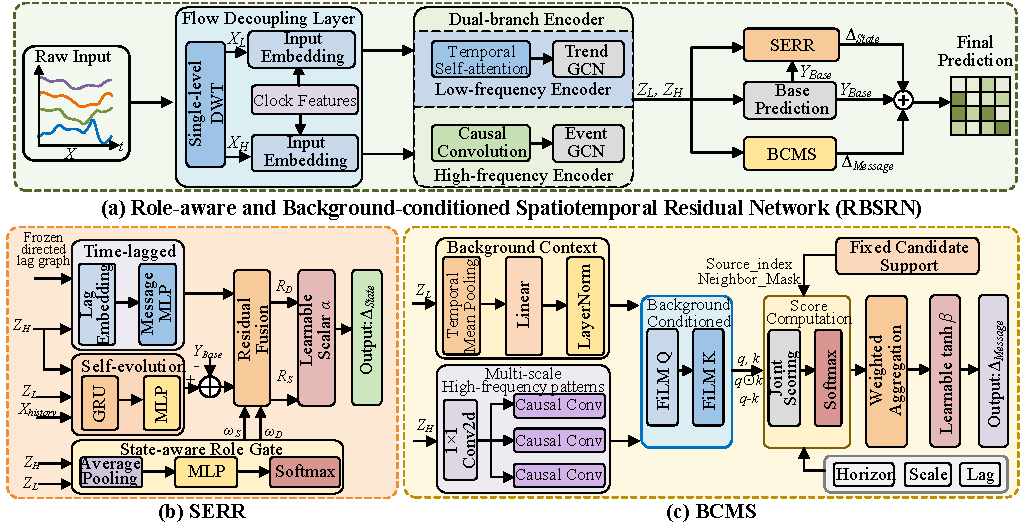
\includegraphics[width=\linewidth]{figures/model-architecture.pdf}
  \caption{\editorialupdated{Overall architecture of RBSRN. (a) Base prediction and parallel residual fusion. (b) SERR expert residual refinement. (c) BCMS background-conditioned historical message selection.}}
  \label{fig:rbsrn-architecture}
\end{figure}

\subsection{Shared Dual-Frequency Spatiotemporal Representations}\label{sec:dual-frequency}

To distinguish smooth changes from short-term fluctuations, RBSRN extracts shared representations through low- and high-frequency branches. We first apply single-level discrete wavelet decomposition and reconstruction along the historical time dimension of each flow channel, producing low- and high-frequency sequences. We standardize both sequences using the channel-wise means and standard deviations of training traffic flow. We then append time-of-day and day-of-week information to obtain \(U_L,U_H\in\mathbb{R}^{T\times N\times4}\). The two branches share the input projection and temporal embeddings. The low-frequency branch applies temporal self-attention and trend graph encoding, whereas the high-frequency branch applies temporal convolution and event graph encoding:
\begin{equation}
\label{eq:low-frequency}
Z_L=\mathrm{F}_L(U_L),
\end{equation}
\begin{equation}
\label{eq:high-frequency}
Z_H=\mathrm{F}_H(U_H),
\end{equation}
where \(Z_L,Z_H\in\mathbb{R}^{T\times N\times d_b}\) and \(d_b\) denotes the shared representation dimension. We fuse the two feature streams using a gated linear unit (GLU) and a rectified linear unit (ReLU) to obtain the base prediction:
\begin{equation}
\label{eq:base-prediction}
\widetilde{Y}^{0}=\mathrm{R}\!\left(\operatorname{ReLU}\!\left[Z_L+\operatorname{GLU}(Z_L)+Z_H\right]\right).
\end{equation}
The convolutional prediction head \(\mathrm{R}\) spans the full historical window and maps the features to inflow and outflow predictions for the next \(H\) steps. SERR and BCMS use \(Z_L\) before the GLU operation, together with \(Z_H\), as their shared inputs.

\subsection{State-Evidence Expert Residual Refinement (SERR)}\label{sec:serr}

SERR organizes two complementary experts around node self-evolution and cross-region time-lagged associations, then allocates their correction contributions according to the current state (Figure~\ref{fig:rbsrn-architecture}(b)). To connect the routine-flow reference with recent dynamics, let \(x_{k,i,c}\) denote the raw flow at historical position \(k\), node \(i\), and channel \(c\). The corresponding routine-flow reference estimated from training data is \(b_{k,i,c}\). We define the state evidence as
\begin{equation}
\label{eq:state-evidence}
\begin{aligned}
\bar{x}_{k,i,c}&=\frac{1}{\ell_k}\sum_{r=k-\ell_k+1}^{k}x_{r,i,c},\qquad \ell_k=\min(3,k),\\
e_{i,c}&=\left[\bar{x}_{T,i,c}-b_{T,i,c},\;x_{T,i,c}-\bar{x}_{T,i,c}\right]^{\mathsf T}.
\end{aligned}
\end{equation}
The two components of \(e_{i,c}\in\mathbb{R}^{2}\) describe trend deviation and short-term fluctuation at the final historical time step, respectively. The mean uses only observed positions within the current historical window and adjusts its length to the available observations at the window's start.

The self-evolution expert encodes recent trajectories within each individual node. For each flow channel, it concatenates the sum of the shared dual-frequency features with raw flow and feeds the result into a shared gated recurrent unit (GRU). It then maps the final hidden state to a multi-step prediction:
\begin{equation}
\label{eq:self-expert}
P^{\mathrm{self}}_{:,i,c}
=\mathcal{P}_{S}\!\left(\psi_S\!\left(\operatorname{GRU}_{\mathrm{last}}
\left([Z_{L,k,i}+Z_{H,k,i}\,\Vert\,x_{k,i,c}]_{k=1}^{T}\right)\right)\right).
\end{equation}
Here, \(\Vert\) denotes feature concatenation, and \(\psi_S\) is a two-layer perceptron with tanh activation. The projection \(\mathcal{P}_S\) linearly maps \(d_b\)-dimensional features to predictions over \(H\) steps. This branch further extracts each node's temporal evolution from the shared spatiotemporal representations.

The directed time-lagged expert retrieves historical features from source nodes through the preconstructed and frozen association set \(\mathcal{E}_c\). For an edge \((j,i,\ell)\in\mathcal{E}_c\), \(j\) is the source node, \(i\) is the target node, and \(\ell\) is a historical lag satisfying \(0<\ell<T\). A lag embedding modulates the source high-frequency features, which are then combined with the target state evidence to form supplementary messages:
\begin{equation}
\label{eq:delay-expert}
\begin{aligned}
\eta_{i,c}&=W_e e_{i,c},\\
m_{j\to i,\ell,c}&=\psi_D\!\left([(1+\tanh v_{\ell})\odot Z_{H,T-\ell,j}\,\Vert\,\eta_{i,c}]\right),\\
R^{\mathrm{delay}}_{:,i,c}&=\mathcal{P}_D\!\left(\eta_{i,c}
+\sum_{(j,i,\ell)\in\mathcal{E}_c}a_{ji\ell}^{c}m_{j\to i,\ell,c}\right).
\end{aligned}
\end{equation}
Here, \(W_e\in\mathbb{R}^{d_b\times2}\) projects the evidence, and \(v_\ell\in\mathbb{R}^{d_b}\) is a learnable lag embedding. The message transformation \(\psi_D\) uses a sigmoid linear unit (SiLU) activation without bias, \(a_{ji\ell}^{c}\) is a fixed edge weight, and \(\mathcal{P}_D\) is a multi-step linear output head. Each expert shares its own parameters across nodes and flow channels, while directed time-lagged associations are specified separately for each flow channel.

A state-conditioned gate determines expert contributions from the temporal means of low- and high-frequency features and the state evidence for both flow channels:
\begin{equation}
\label{eq:role-gate}
\Omega_i=\operatorname{Softmax}_{\mathrm{expert}}\!\left(
\operatorname{reshape}_{2\times2}\,g\!\left(
[\bar{Z}_{L,i}\,\Vert\,\bar{Z}_{H,i}\,\Vert\,e_{i,\mathrm{in}}\,\Vert\,e_{i,\mathrm{out}}]
\right)\right).
\end{equation}
The temporal means \(\bar{Z}_{L,i},\bar{Z}_{H,i}\) are \(d_b\)-dimensional vectors averaged over the historical window, and \(g\) is a two-layer perceptron with SiLU activation. In \(\Omega_i\in\mathbb{R}^{2\times2}\), rows correspond to flow channels, and columns correspond to the self-evolution and directed time-lagged experts. Softmax normalizes along the expert dimension to produce \(\omega^S_{i,c}\) and \(\omega^D_{i,c}\). These weights vary by sample, node, and flow channel but are shared across all forecast steps. The resulting residual correction is
\begin{equation}
\label{eq:serr-residual}
\Delta\widetilde{Y}^{S}_{h,i,c}
=\alpha\left[\omega^S_{i,c}\left(P^{\mathrm{self}}_{h,i,c}-\widetilde{Y}^{0}_{h,i,c}\right)
+\omega^D_{i,c}R^{\mathrm{delay}}_{h,i,c}\right].
\end{equation}
Both \(P^{\mathrm{self}}\) and \(R^{\mathrm{delay}}\) use the same standardized flow scale as the base prediction, and \(\alpha\) is a global learnable scalar. The self-evolution expert contributes a residual relative to the base prediction, whereas the directed time-lagged expert provides a correction from cross-region historical information. The state-conditioned gate combines the contributions of these two experts.

\subsection{Background-conditioned Cross-region Message Selection (BCMS)}\label{sec:bcms}

BCMS selects historical messages within fixed candidate neighborhoods according to the current background and forecast horizon (Figure~\ref{fig:rbsrn-architecture}(c)). It first maps the temporal mean of low-frequency features to a node background representation and extracts multiscale patterns from high-frequency features:
\begin{equation}
\label{eq:bcms-context-pattern}
\xi_i=\operatorname{LN}\!\left(\mathcal{P}_b(\bar{Z}_{L,i})\right),
\qquad z^s=\mathcal{T}_s\!\left(\mathcal{P}_H(Z_H)\right).
\end{equation}
Here, \(\xi_i\in\mathbb{R}^{d}\) and \(z^s\in\mathbb{R}^{T\times N\times d}\), with \(d=32\). The operator \(\mathcal{P}_b\) is a linear projection, LN denotes layer normalization, and \(\mathcal{P}_H\) is a \(1\times1\) convolution shared across scales. Each \(\mathcal{T}_s\) consists of a left-padded depthwise temporal convolution, a pointwise convolution, and a Gaussian error linear unit (GELU) activation. The three scales use a kernel size of 3 and dilation rates of 1, 2, and 4, yielding temporal spans \(r_s\in\{3,5,9\}\).

For node \(i\), let \(\mathcal{N}_i\) denote its fixed candidate source set and consider historical lags \(\tau\in\{0,1,2,3\}\). The valid candidate set is \(\mathcal{A}_i=\{(j,\tau,s):j\in\mathcal{N}_i,\ r_s+\tau\leq T\}\), with at most 8 sources retained per node. At each scale, the query represents the target's final historical pattern, and the key represents a source historical pattern. Their respective low-frequency backgrounds modulate the query and key:
\begin{equation}
\label{eq:background-conditioned-qk}
\begin{aligned}
q_i^s&=(1+\gamma_q(\xi_i))\odot Q(z^s_{T,i})+\delta_q(\xi_i),\\
k_{j,\tau}^s&=(1+\gamma_k(\xi_j))\odot K(z^s_{T-\tau,j})+\delta_k(\xi_j).
\end{aligned}
\end{equation}
The operators \(Q,K\) are learnable affine mappings; \(\gamma\) and \(\delta\) produce \(d\)-dimensional scaling and shifting parameters, respectively~\cite{ref45}. Thus, both source and target low-frequency traffic backgrounds condition the matching of high-frequency patterns.

For forecast step \(h\), we define the joint score as
\begin{equation}
\label{eq:joint-message-score}
\begin{aligned}
u_{i,j,\tau,s}
&=A_q q_i^s+A_k k_{j,\tau}^s
+A_p(q_i^s\odot k_{j,\tau}^s)+A_d(q_i^s-k_{j,\tau}^s)+b_a,\\
a_{h,i,j,\tau,s}
&=w_a^{\mathsf T}\operatorname{GELU}\!\left(
u_{i,j,\tau,s}+e_{\mathrm{lag}}(\tau)+e_{\mathrm{scale}}(r_s)+e_{\mathrm{hor}}(h)\right).
\end{aligned}
\end{equation}
Here, \(A_q,A_k,A_p,A_d\in\mathbb{R}^{d\times d}\) and \(b_a,w_a\in\mathbb{R}^{d}\) are learnable parameters. Each of the three temporal encodings applies a bias-free linear projection to \([v,\sin(2\pi v),\cos(2\pi v)]^{\mathsf T}\). The value \(v\) expresses the corresponding historical lag, temporal span, or forecast horizon in hours. Introducing the forecast-step encoding before nonlinear scoring allows candidate contributions to vary with the forecast horizon.

To control the overall contribution of historical information, we add a zero-message option with both score and value set to zero at each forecast step. For each actual candidate, joint normalization gives the weight
\begin{equation}
\label{eq:joint-message-softmax}
w_{h,i,j,\tau,s}
=\frac{\exp(a_{h,i,j,\tau,s})}
{1+\displaystyle\sum_{(j',\tau',s')\in\mathcal{A}_i}\exp(a_{h,i,j',\tau',s'})}.
\end{equation}
The denominator's constant 1 corresponds to the zero-message option. Its probability mass allows the model to reduce the total weight assigned to actual historical messages. We project the source high-frequency patterns to values, aggregate them with the selection weights, and generate corrections for both flow channels:
\begin{equation}
\label{eq:bcms-residual}
\begin{aligned}
m_{h,i}&=\sum_{(j,\tau,s)\in\mathcal{A}_i}
w_{h,i,j,\tau,s}W_vz^s_{T-\tau,j},\\
\Delta\widetilde{Y}^{B}_{h,i,:}&=\tanh(\beta)\,W_o m_{h,i}.
\end{aligned}
\end{equation}
Both \(W_v\in\mathbb{R}^{d\times d}\) and \(W_o\in\mathbb{R}^{2\times d}\) are bias-free projections, and \(\beta\) is a global learnable scalar. Inflow and outflow share the message selection weights and aggregated representation, while the two-output head produces their respective corrections. BCMS generates weights for each forecast step, complementing the SERR expert weights shared across forecast steps.

\subsection{Joint Forecasting Output}\label{sec:joint-output}

We add both corrections to the base prediction according to Eq.~\eqref{eq:overall-prediction}. We then restore the original traffic flow scale using fixed channel-wise statistics estimated from training input windows:
\begin{equation}
\label{eq:inverse-scaling}
\widehat{Y}_{t+h,i,c}
=\sigma_c\left(\widetilde{Y}^{0}_{h,i,c}
+\Delta\widetilde{Y}^{S}_{h,i,c}+\Delta\widetilde{Y}^{B}_{h,i,c}\right)+\mu_c.
\end{equation}
Here, \(\mu_c\) and \(\sigma_c\) denote the mean and standard deviation of channel \(c\), respectively. We initialize both global correction-strength parameters, \(\alpha\) and \(\beta\), to zero, so the initial output equals the base prediction. We also zero-initialize the final SERR gating layer, giving both experts an initial weight of 0.5. The model then learns the contributions of the two complementary correction pathways under a joint inflow and outflow forecasting objective.

% !TeX root = ../main.tex
% !TeX encoding = UTF-8
% !TeX spellcheck = none
\section{Experiments and Analysis}\label{sec:experiments}

\subsection{Experimental Settings}\label{sec:exp-settings}

\subsubsection{Datasets, Preprocessing, and Forecasting Protocol}\label{sec:exp-datasets}

We evaluated regional traffic flow forecasting on two datasets: Chengdu DiDi ride-hailing orders collected in November 2016 and Shanghai taxi origin--destination (OD) records collected in August 2016. For each city, we selected a fixed core area and divided it into a \(32\times32\) grid. Inflow and outflow are counts per 5 min, aggregated independently from trip destinations and origins, respectively. Table~\ref{tab:dataset-summary} summarizes the datasets, and Figures~\ref{fig:chengdu-t5-dataset} and~\ref{fig:shanghai-t5-dataset} show their endpoint distributions, grid partitions, and mean flows.

Both datasets used the same cleaning and aggregation procedure, with timestamps converted to Beijing time (UTC+8). We removed exact duplicates and records with invalid timestamps or coordinates. Retained orders lasted 2--120 minutes, had both endpoints within the city's coarse geographic boundary, and had an average speed no greater than \(120\,\mathrm{km/h}\), computed from great-circle distance and trip duration. Valid endpoints in the core area were aggregated into grid cells and time intervals; cells with no endpoint events were assigned zero. Shanghai source quality was flagged as invalid from 2016-08-11 to 2016-08-14. We retained these records in the flow series and in the training-input statistics, while applying the quality mask when computing source-quality summaries and scenario references.

\begin{table}[!htbp]
	\centering
	\caption{Dataset properties and sample splits}
	\label{tab:dataset-summary}
	\small
	\begin{tabular}{lcc}
		\toprule
		Property & Chengdu & Shanghai \\
		\midrule
		Observation period & 2016-11-01 to 2016-11-30 & 2016-08-01 to 2016-08-31 \\
		Grid size & \(32\times32\) & \(32\times32\) \\
		Approx. cell dimensions (km) & \(0.42\times0.44\) & \(0.80\times0.68\) \\
		Sampling interval & 5 minutes & 5 minutes \\
		Complete time intervals & 8,640 & 8,928 \\
		Orders after cleaning & 6,082,753 & 7,744,423 \\
		Training windows & 5,170 & 5,343 \\
		Validation windows & 1,724 & 1,781 \\
		Test windows & 1,723 & 1,781 \\
		\bottomrule
	\end{tabular}
\end{table}

For each dataset, we generated stride-1 rolling-origin windows. Each window uses the past 12 observations to predict inflow and outflow over the next 12 steps, covering 60 minutes of history and forecasts. We retained the associated time-of-day and day-of-week features and kept only windows with complete inputs and targets. The resulting windows were ordered by forecast origin and divided chronologically into training, validation, and test sets at an approximate ratio of 6:2:2 (Table~\ref{tab:dataset-summary}). This rolling-origin protocol preserves temporal order while allowing each forecast origin to use the immediately preceding observations as history. All methods used the same ordered indices and forecasting task.

For each flow channel, standardization means and standard deviations were computed from the historical inputs of training windows and fixed for validation and testing. Predictions were returned to the original flow scale by channel-wise inverse standardization. Section~\ref{sec:exp-implementation} describes checkpoint selection, and Section~\ref{sec:exp-baselines-metrics} defines the evaluation metrics.

\begin{figure}[!htbp]
	\centering
	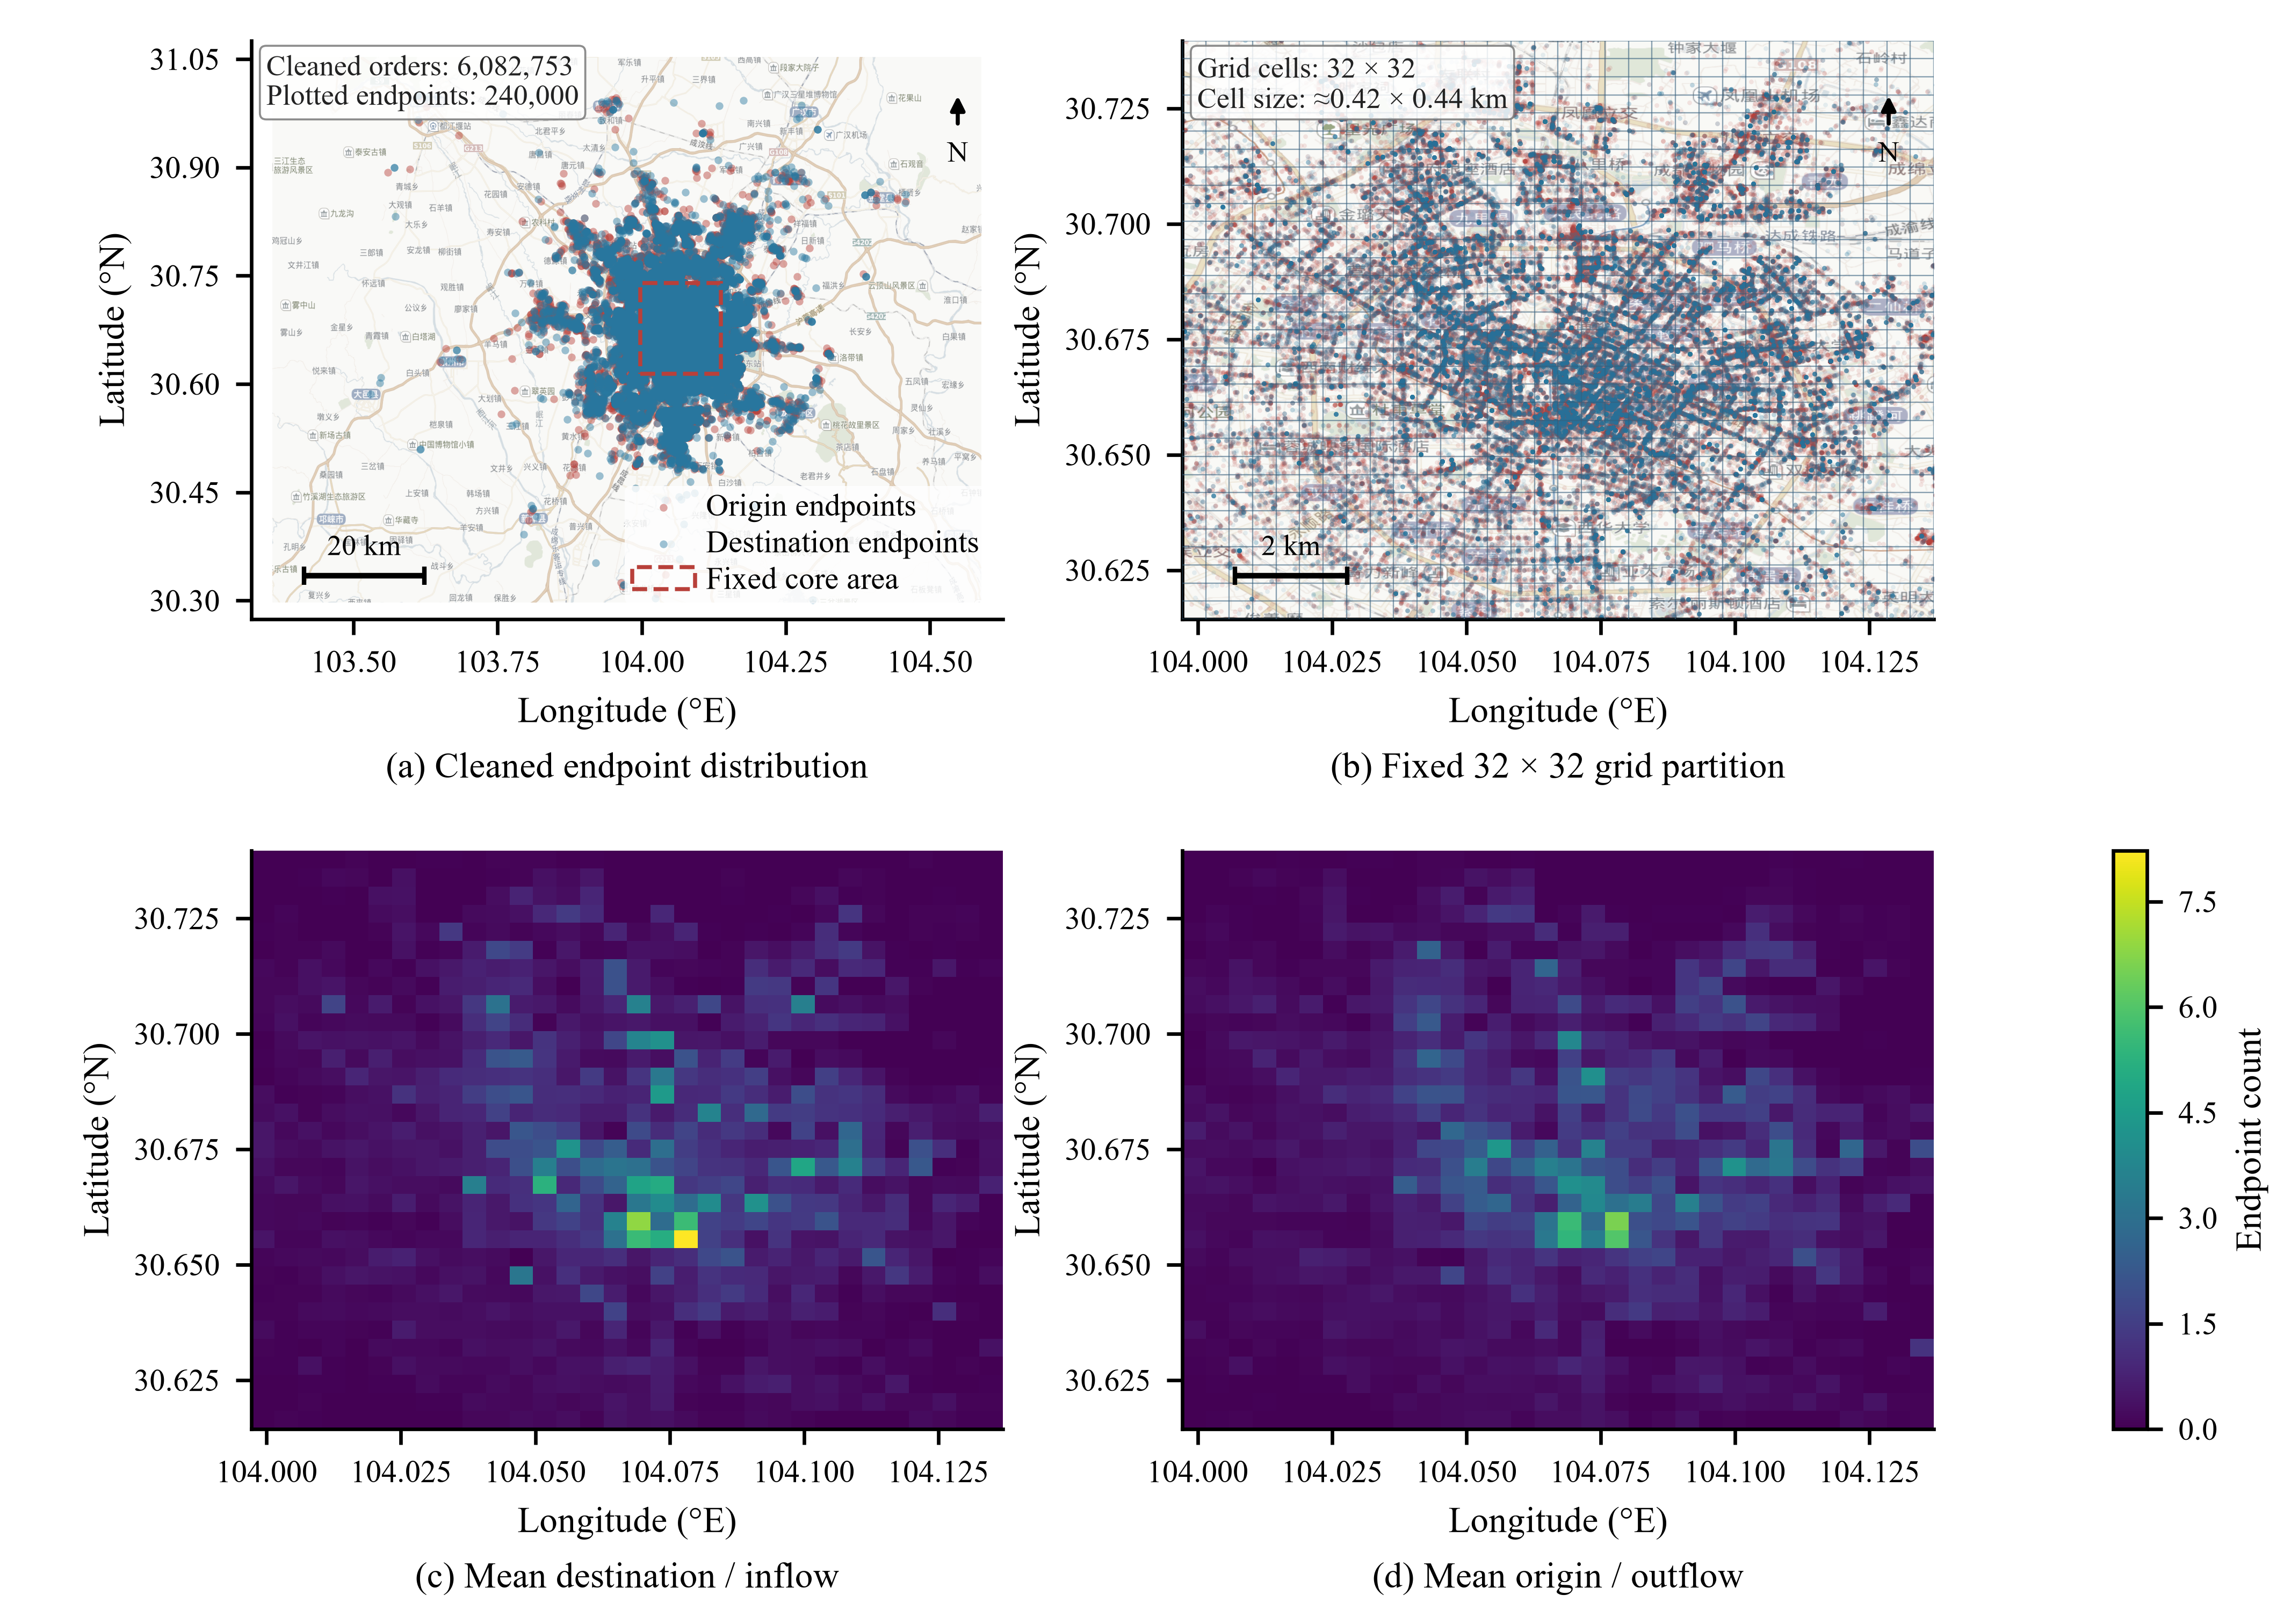
\includegraphics[width=\linewidth]{figures/chengdu-t5-overview.png}
\caption{Chengdu endpoint distribution, grid partition, and mean flow.}
	\label{fig:chengdu-t5-dataset}
\end{figure}

\begin{figure}[!htbp]
	\centering
	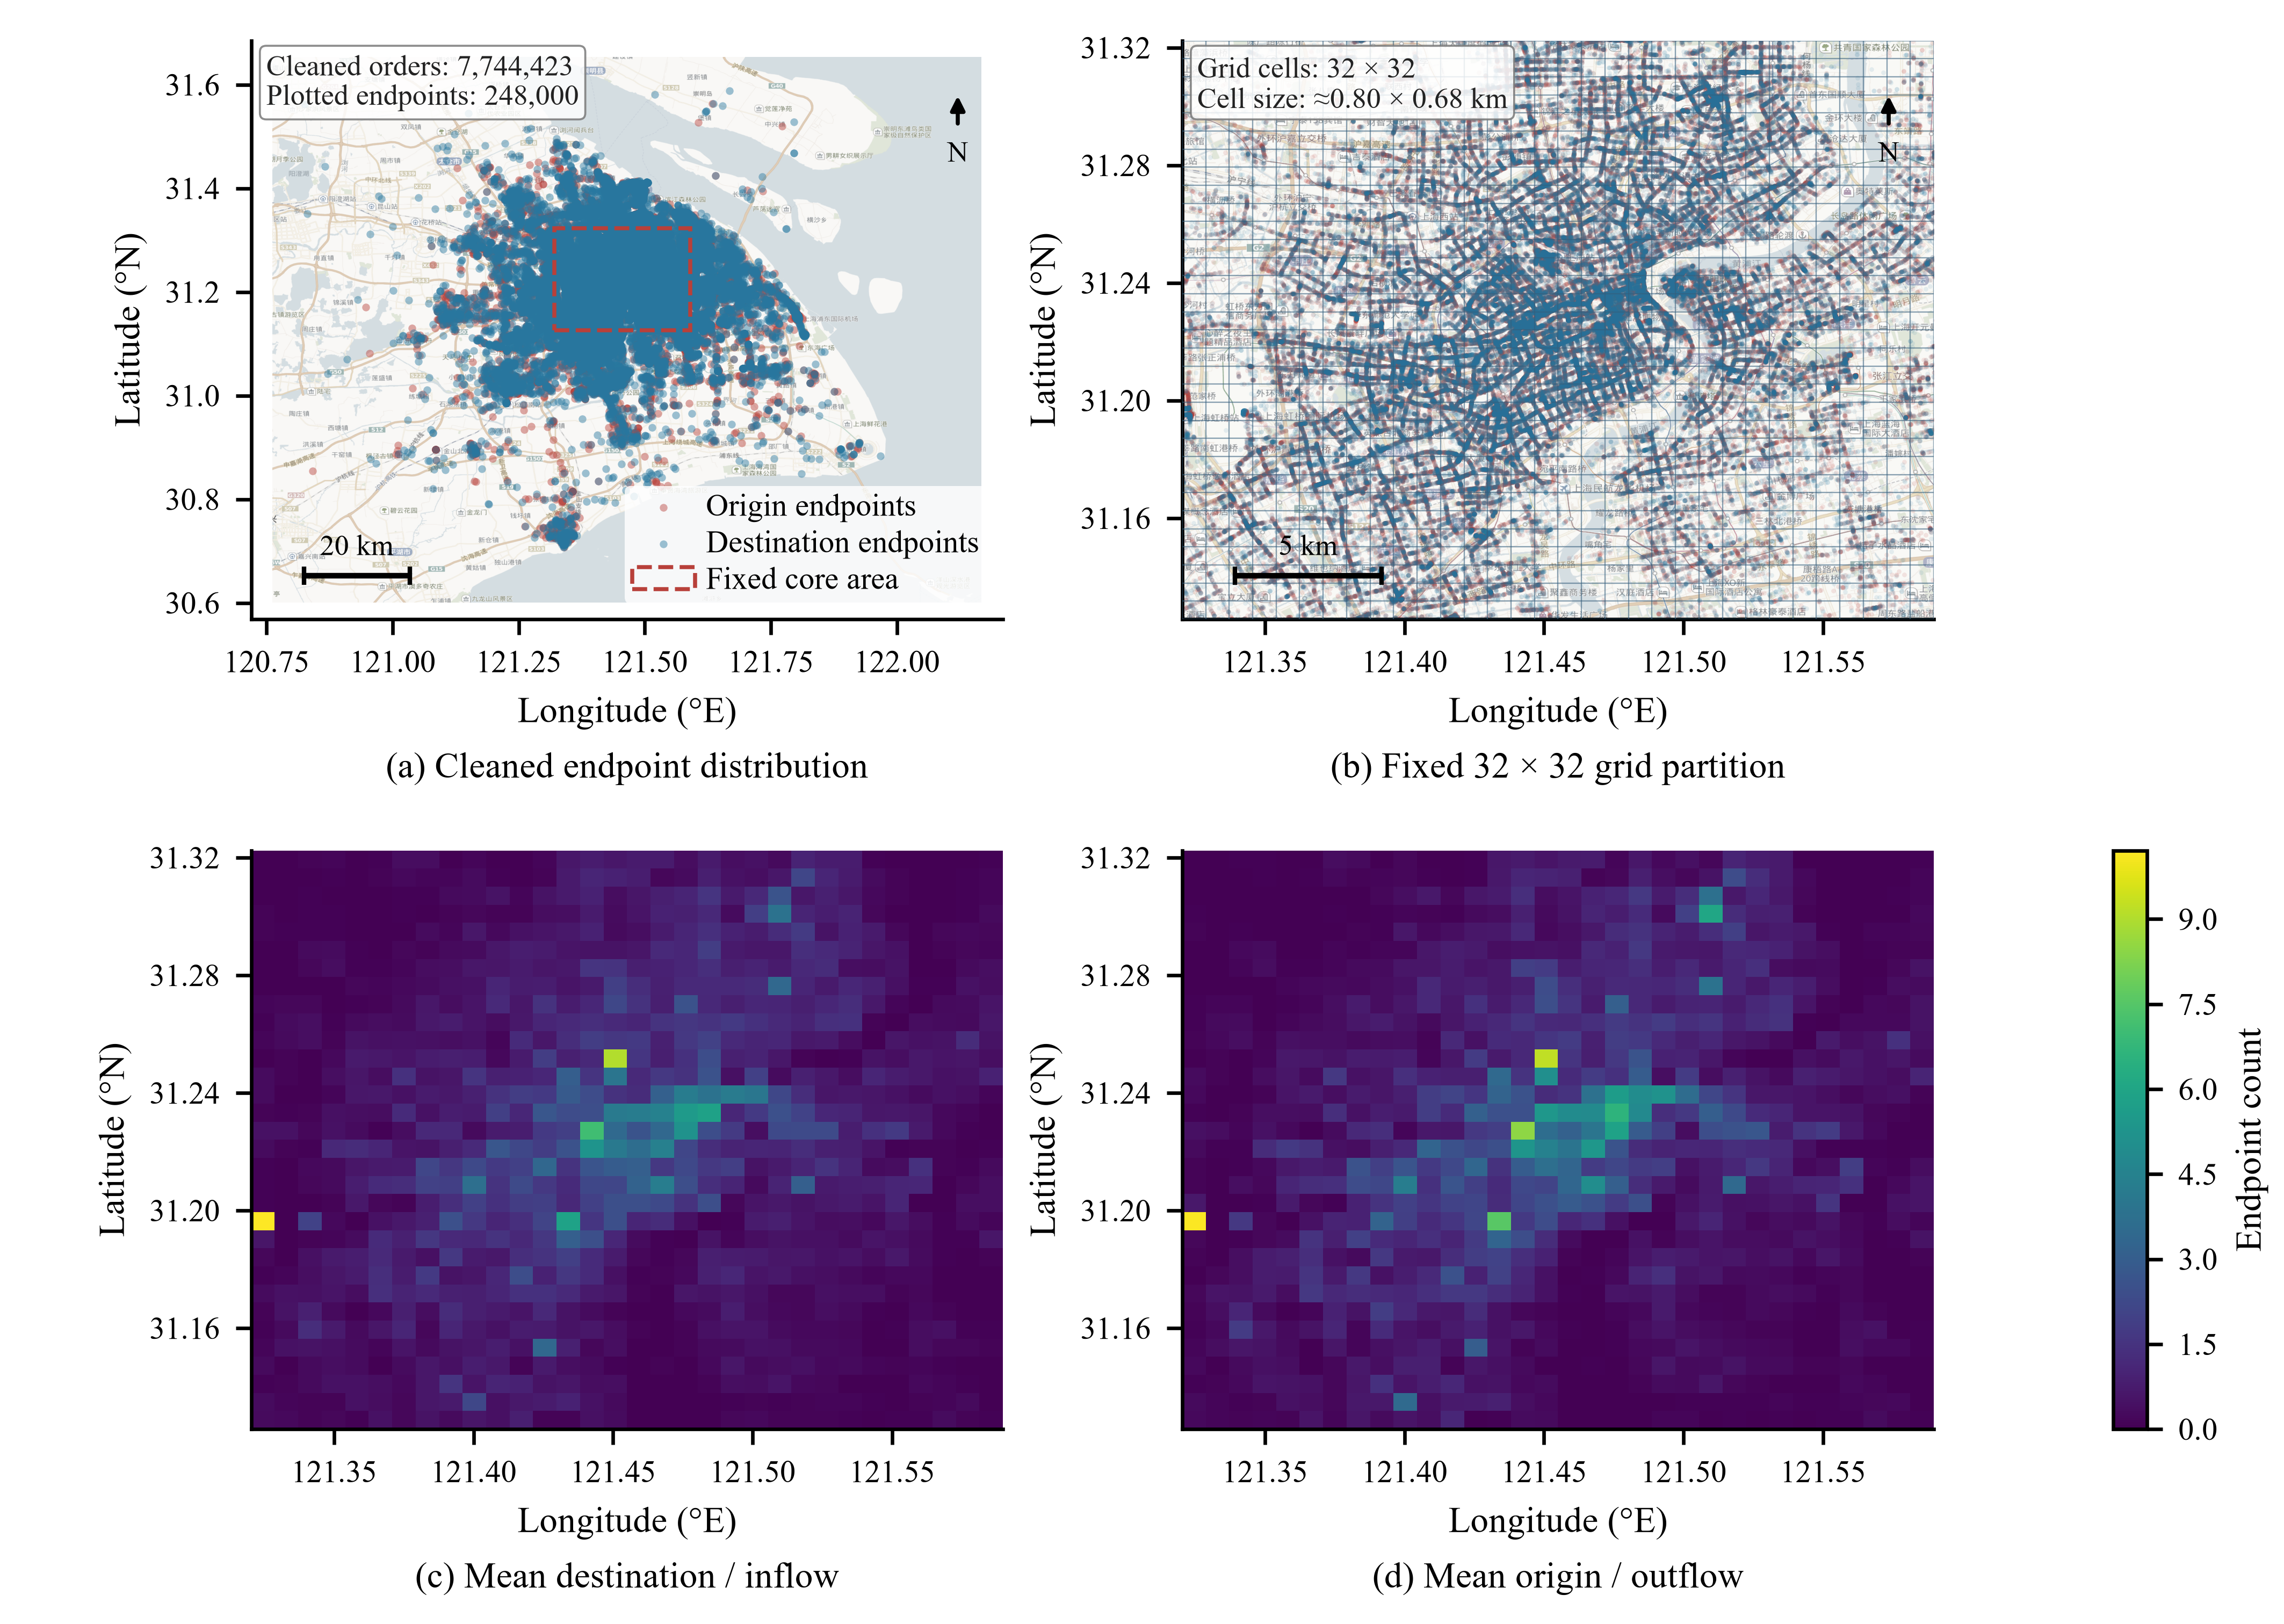
\includegraphics[width=\linewidth]{figures/shanghai-t5-overview.png}
\caption{Shanghai endpoint distribution, grid partition, and mean flow.}
	\label{fig:shanghai-t5-dataset}
\end{figure}

\subsubsection{Baseline Methods and Evaluation Metrics}\label{sec:exp-baselines-metrics}

The main experiments compared RBSRN with 13 baselines from three forecasting paradigms. Conventional methods were historical average (HA) and support vector regression (SVR). Deep models were DCRNN~\cite{ref01}, STGCN~\cite{ref02}, Graph WaveNet (GWNet)~\cite{ref03}, DSTAGNN~\cite{ref19}, PDFormer~\cite{ref10}, STDN~\cite{ref20}, MetaDG~\cite{ref21}, HyperD~\cite{ref22}, and RAST~\cite{ref23}; general time-series models were PatchTST~\cite{ref12} and TimeMixer~\cite{ref13}. Every method used the chronological split and 12-step task defined above. Inflow and outflow were evaluated separately in each city.

The scenario analysis additionally included vector autoregression (VAR), STNorm~\cite{ref24}, and STWave~\cite{ref11}, for 16 baselines in total.

We use mean absolute error (MAE) and root mean squared error (RMSE), computed on the original flow scale after inverse standardization. The main tables use a positive-target mask and evaluate locations with observed flow greater than zero. The scope-sensitivity analysis applies the same RBSRN checkpoint to all grid cells, including zero targets; it characterizes metric sensitivity rather than reranking baselines. Let \(\mathcal{T}_{\mathrm{test}}\) denote the forecast origins of the actual test windows. Let \(y_{t,h,i,c}\) and \(\widehat y_{t,h,i,c}\) denote the observed and predicted values for forecast origin \(t\), forecast step \(h\), grid cell \(i\), and channel \(c\in\{\mathrm{in},\mathrm{out}\}\). The prediction error is \(e_{t,h,i,c}=\widehat y_{t,h,i,c}-y_{t,h,i,c}\). The two evaluation scopes are
\[
\begin{aligned}
	\Omega^{+}_{h,c}&=\bigl\{(t,i)\mid t\in\mathcal{T}_{\mathrm{test}},\ 1\leq i\leq N,\ y_{t,h,i,c}>0\bigr\},\\
	\Omega^{\mathrm{all}}_{h,c}&=\mathcal{T}_{\mathrm{test}}\times\{1,\ldots,N\}.
\end{aligned}
\]
For \(m\in\{+,\mathrm{all}\}\), we pool all test windows and nodes within the corresponding scope to compute
\begin{equation}
	\label{eq:eval-mae}
	\mathrm{MAE}^{m}_{h,c}
	=\frac{1}{|\Omega^{m}_{h,c}|}
	\sum_{(t,i)\in\Omega^{m}_{h,c}}|e_{t,h,i,c}|,
\end{equation}
\begin{equation}
	\label{eq:eval-rmse}
	\mathrm{RMSE}^{m}_{h,c}
	=\sqrt{\frac{1}{|\Omega^{m}_{h,c}|}
		\sum_{(t,i)\in\Omega^{m}_{h,c}}e_{t,h,i,c}^{2}}.
\end{equation}
Here, \(|\Omega^{m}_{h,c}|\) is the number of evaluated locations. Both scopes exclude duplicate windows introduced by test-batch padding, and inflow and outflow are evaluated separately.

We report the single-step results H3, H6, and H12, corresponding to forecast steps 3, 6, and 12, or forecast horizons of 15, 30, and 60 minutes. AVG12 denotes the arithmetic mean of the metrics over all 12 forecast steps:
\begin{equation}
	\label{eq:eval-avg12}
	\mathrm{AVG12}\text{-}\mathcal{M}^{m}_{c}
	=\frac{1}{12}\sum_{h=1}^{12}\mathcal{M}^{m}_{h,c},
	\qquad\mathcal{M}\in\{\mathrm{MAE},\mathrm{RMSE}\}.
\end{equation}
For AVG12 RMSE, we compute RMSE at each forecast step and then average those 12 values.

\FloatBarrier

\textbf{}% !TeX root = ../main.tex
\subsubsection{Implementation and Computing Environment}\label{sec:exp-implementation}

Model experiments used a single NVIDIA A100-SXM4-40GB GPU. Table~\ref{tab:hyperparameter-implementation} lists the hardware, software, and training settings. All configurations used the same data split, a maximum of 200 epochs, and an early-stopping patience of 20 epochs. We selected the checkpoint with the lowest joint validation MAE and reported MAE and RMSE at that checkpoint.

% !TeX root = ../main.tex
\begin{table}[!htbp]
  \centering
  \caption[RBSRN computing environment and training settings]{\hpupdated{Model computing environment and training settings}}
  \label{tab:hyperparameter-implementation}
  \small
  \renewcommand{\arraystretch}{1.12}
  \begin{tabular}{@{}p{0.25\linewidth}p{0.69\linewidth}@{}}
    \toprule
    Item & Setting \\
    \midrule
    Optimizer and learning rate & Ranger; fixed at 0.001, with no learning-rate schedule \\
    Weight decay & \(10^{-4}\); no decay for the BCMS parameter \(\beta\) \\
    Batch size & 64 for both training and validation \\
    Training budget and checkpoint selection & At most 200 epochs, with an early-stopping patience of 20 epochs; checkpoint selected by the lowest joint validation MAE \\
    \midrule
    GPU & One NVIDIA A100-SXM4-40GB, with 40 GB of GPU memory \\
    CPU & Two Intel Xeon Gold 6138 processors @ 2.00 GHz, with 40 cores and 80 threads in total \\
    Software environment & Python 3.11.15; PyTorch 2.7.1+cu128; CUDA 12.8 (PyTorch build version) \\
    \bottomrule
  \end{tabular}
\end{table}



% !TeX root = ../main.tex
% !TeX encoding = UTF-8
% !TeX spellcheck = none
\subsection{Main Experimental Results}\label{sec:exp-main-results}

This section evaluates RBSRN in terms of overall prediction accuracy, spatial distributions, deviations from routine patterns, and the effects of residual corrections. Comparisons across the full test set and fixed-model diagnostics examine how the two types of correction evidence perform under different traffic conditions.

\subsubsection{Overall Prediction Performance}\label{sec:results-overall}

Tables~\ref{tab:chengdu-inflow}--\ref{tab:shanghai-outflow} compare RBSRN with 13 baseline methods on inflow and outflow forecasting in Chengdu and Shanghai, using positive-target evaluation. Relative changes were calculated from unrounded values against the strongest baseline method for each task and metric. \editorialupdated{Bold and underlined values indicate the best and second-best results in each column, respectively.}

\shanghaiupdated{RBSRN achieved the lowest AVG12 MAE and RMSE on all four tasks. For Chengdu inflow, Chengdu outflow, Shanghai inflow, and Shanghai outflow, AVG12 MAE decreased by 2.00\%, 0.46\%, 1.18\%, and 0.43\% relative to each task's strongest baseline method. AVG12 RMSE decreased by 5.01\%, 1.50\%, 2.33\%, and 0.06\%, respectively, with STGCN, STGCN, HyperD, and HyperD as the corresponding strongest baseline methods.}

Across forecast horizons, RBSRN achieved the lowest MAE and RMSE at H3, H6, and H12 for inflow forecasting in both cities. \shanghaiupdated{For outflow forecasting, HyperD achieved the best H12 MAE in both cities and the best H12 RMSE in Shanghai. RBSRN achieved the lowest errors in all remaining reported comparisons.}

% !TeX root = ../main.tex
% !TeX spellcheck = none
\begin{table}[!htbp]
\centering
\caption{Inflow forecasting results for Chengdu (\(32\times32\) grid)}
\label{tab:chengdu-inflow}
\begingroup
\linespread{1}\fontsize{10}{12}\selectfont
\setlength{\tabcolsep}{4.5pt}
\renewcommand{\arraystretch}{1.05}
\begin{tabular*}{\linewidth}{@{\extracolsep{\fill}}l*{8}{r}@{}}
\toprule
& \multicolumn{2}{c}{H3} & \multicolumn{2}{c}{H6} & \multicolumn{2}{c}{H12} & \multicolumn{2}{c}{AVG12} \\
\cmidrule(l{4.5pt}r{4.5pt}){2-3}\cmidrule(l{4.5pt}r{4.5pt}){4-5}\cmidrule(l{4.5pt}r{4.5pt}){6-7}\cmidrule(l{4.5pt}r{4.5pt}){8-9}
Model & MAE & RMSE & MAE & RMSE & MAE & RMSE & MAE & RMSE \\
\midrule
HA & 1.053 & 1.522 & 1.083 & 1.600 & 1.144 & 1.739 & 1.088 & 1.609 \\
SVR & 0.810 & 1.354 & 0.835 & 1.391 & 0.892 & 1.499 & 0.840 & 1.405 \\
DCRNN (ICLR'18) & 0.725 & \underline{1.321} & 0.790 & 1.363 & 1.025 & 1.574 & 0.829 & 1.399 \\
STGCN (IJCAI'18) & 0.721 & 1.342 & 0.724 & \underline{1.348} & 0.743 & 1.409 & 0.728 & \underline{1.362} \\
GWNet (IJCAI'19) & \underline{0.719} & 1.332 & 0.731 & 1.373 & 0.756 & 1.450 & 0.733 & 1.378 \\
DSTAGNN (ICML'22) & 1.022 & 1.461 & 1.008 & 1.458 & 1.044 & 1.505 & 1.027 & 1.473 \\
PDFormer (AAAI'23) & \pdformerupdated{1.002} & \pdformerupdated{1.443} & \pdformerupdated{1.013} & \pdformerupdated{1.473} & \pdformerupdated{1.030} & \pdformerupdated{1.515} & \pdformerupdated{1.014} & \pdformerupdated{1.473} \\
PatchTST (ICLR'23) & 0.799 & 1.405 & 0.826 & 1.483 & 0.880 & 1.614 & 0.831 & 1.490 \\
TimeMixer (ICLR'24) & 0.818 & 1.434 & 0.844 & 1.505 & 0.895 & 1.620 & 0.848 & 1.510 \\
STDN (AAAI'25) & 1.178 & 1.589 & 1.180 & 1.593 & 1.179 & 1.600 & 1.178 & 1.593 \\
MetaDG (AAAI'26) & 1.102 & 1.564 & 1.170 & 1.678 & 1.291 & 1.882 & 1.178 & 1.692 \\
HyperD (AAAI'26) & 0.723 & 1.369 & \underline{0.723} & 1.369 & \underline{0.726} & \underline{1.382} & \underline{0.723} & 1.369 \\
RAST (AAAI'26) & 0.724 & 1.332 & 0.734 & 1.372 & 0.756 & 1.446 & 0.736 & 1.377 \\
\midrule
\textbf{RBSRN (Ours)} & \textbf{0.704} & \textbf{1.282} & \textbf{0.707} & \textbf{1.290} & \textbf{0.717} & \textbf{1.318} & \textbf{0.708} & \textbf{1.294} \\
\bottomrule
\end{tabular*}
\endgroup
\end{table}

% !TeX root = ../main.tex
% !TeX spellcheck = none
\begin{table}[!htbp]
\centering
\caption{Outflow forecasting results for Chengdu (\(32\times32\) grid)}
\label{tab:chengdu-outflow}
\begingroup
\linespread{1}\fontsize{10}{12}\selectfont
\setlength{\tabcolsep}{4.5pt}
\renewcommand{\arraystretch}{1.05}
\begin{tabular*}{\linewidth}{@{\extracolsep{\fill}}l*{8}{r}@{}}
\toprule
& \multicolumn{2}{c}{H3} & \multicolumn{2}{c}{H6} & \multicolumn{2}{c}{H12} & \multicolumn{2}{c}{AVG12} \\
\cmidrule(l{4.5pt}r{4.5pt}){2-3}\cmidrule(l{4.5pt}r{4.5pt}){4-5}\cmidrule(l{4.5pt}r{4.5pt}){6-7}\cmidrule(l{4.5pt}r{4.5pt}){8-9}
Model & MAE & RMSE & MAE & RMSE & MAE & RMSE & MAE & RMSE \\
\midrule
HA & 1.023 & 1.404 & 1.043 & 1.439 & 1.085 & 1.510 & 1.047 & 1.445 \\
SVR & 0.792 & 1.239 & 0.809 & 1.251 & 0.838 & 1.285 & 0.810 & 1.255 \\
DCRNN (ICLR'18) & 0.714 & \underline{1.230} & 0.761 & \underline{1.237} & 1.151 & 1.642 & 0.844 & 1.326 \\
STGCN (IJCAI'18) & 0.714 & 1.235 & 0.716 & 1.239 & 0.725 & 1.258 & 0.718 & \underline{1.242} \\
GWNet (IJCAI'19) & 0.713 & 1.253 & 0.718 & 1.265 & 0.729 & 1.289 & 0.719 & 1.267 \\
DSTAGNN (ICML'22) & 1.018 & 1.383 & 1.007 & 1.376 & 1.035 & 1.410 & 1.021 & 1.390 \\
PDFormer (AAAI'23) & \pdformerupdated{0.987} & \pdformerupdated{1.365} & \pdformerupdated{0.990} & \pdformerupdated{1.374} & \pdformerupdated{0.997} & \pdformerupdated{1.391} & \pdformerupdated{0.990} & \pdformerupdated{1.374} \\
PatchTST (ICLR'23) & 0.786 & 1.300 & 0.802 & 1.333 & 0.837 & 1.396 & 0.805 & 1.337 \\
TimeMixer (ICLR'24) & 0.807 & 1.315 & 0.823 & 1.345 & 0.856 & 1.404 & 0.826 & 1.349 \\
STDN (AAAI'25) & 1.135 & 1.501 & 1.135 & 1.501 & 1.135 & 1.503 & 1.134 & 1.500 \\
MetaDG (AAAI'26) & 1.082 & 1.471 & 1.139 & 1.543 & 1.245 & 1.672 & 1.146 & 1.550 \\
HyperD (AAAI'26) & \underline{0.712} & 1.249 & \underline{0.712} & 1.249 & \textbf{0.714} & \underline{1.254} & \underline{0.712} & 1.249 \\
RAST (AAAI'26) & 0.718 & 1.242 & 0.724 & 1.257 & 0.735 & 1.282 & 0.724 & 1.258 \\
\midrule
\textbf{RBSRN (Ours)} & \textbf{0.706} & \textbf{1.220} & \textbf{0.708} & \textbf{1.222} & \underline{0.715} & \textbf{1.234} & \textbf{0.709} & \textbf{1.223} \\
\bottomrule
\end{tabular*}
\endgroup
\end{table}

% !TeX root = ../main.tex
% !TeX spellcheck = none
\begin{table}[!htbp]
\centering
\caption{Inflow forecasting results for Shanghai (\(32\times32\) grid)}
\label{tab:shanghai-inflow}
\begingroup
\linespread{1}\fontsize{10}{12}\selectfont
\setlength{\tabcolsep}{4.5pt}
\renewcommand{\arraystretch}{1.05}
\begin{tabular*}{\linewidth}{@{\extracolsep{\fill}}l*{8}{r}@{}}
\toprule
& \multicolumn{2}{c}{H3} & \multicolumn{2}{c}{H6} & \multicolumn{2}{c}{H12} & \multicolumn{2}{c}{AVG12} \\
\cmidrule(l{4.5pt}r{4.5pt}){2-3}\cmidrule(l{4.5pt}r{4.5pt}){4-5}\cmidrule(l{4.5pt}r{4.5pt}){6-7}\cmidrule(l{4.5pt}r{4.5pt}){8-9}
Model & MAE & RMSE & MAE & RMSE & MAE & RMSE & MAE & RMSE \\
\midrule
HA & 1.019 & 1.437 & 1.040 & 1.490 & 1.080 & 1.593 & 1.043 & 1.498 \\
SVR & 0.817 & 1.251 & 0.837 & 1.274 & 0.879 & 1.344 & 0.841 & 1.283 \\
DCRNN (ICLR'18) & \underline{0.734} & \underline{1.243} & 0.748 & 1.262 & 0.808 & 1.328 & 0.758 & 1.272 \\
STGCN (IJCAI'18) & 0.741 & 1.257 & 0.743 & 1.260 & 0.754 & 1.293 & 0.745 & 1.268 \\
GWNet (IJCAI'19) & 0.735 & 1.268 & 0.742 & 1.288 & 0.760 & 1.343 & 0.744 & 1.295 \\
DSTAGNN (ICML'22) & 1.010 & 1.410 & 0.950 & 1.360 & 1.009 & 1.426 & 0.994 & 1.402 \\
PDFormer (AAAI'23) & \pdformerupdated{0.970} & \pdformerupdated{1.356} & \pdformerupdated{0.977} & \pdformerupdated{1.369} & \pdformerupdated{0.995} & \pdformerupdated{1.413} & \pdformerupdated{0.979} & \pdformerupdated{1.376} \\
PatchTST (ICLR'23) & 0.800 & 1.333 & 0.816 & 1.382 & 0.849 & 1.480 & 0.819 & 1.392 \\
TimeMixer (ICLR'24) & 0.821 & 1.331 & 0.836 & 1.372 & 0.868 & 1.463 & 0.839 & 1.381 \\
STDN (AAAI'25) & 1.219 & 1.651 & 1.220 & 1.659 & 1.219 & 1.683 & 1.218 & 1.661 \\
MetaDG (AAAI'26) & 1.082 & 1.517 & 1.168 & 1.624 & 1.421 & 1.944 & 1.201 & 1.667 \\
HyperD (AAAI'26) & 0.737 & 1.261 & \underline{0.737} & 1.261 & \underline{0.737} & \underline{1.263} & \underline{0.737} & \underline{1.260} \\
RAST (AAAI'26) & 0.736 & 1.245 & 0.740 & \underline{1.259} & 0.749 & 1.289 & 0.741 & 1.261 \\
\midrule
\textbf{RBSRN (Ours)} & \shanghaiupdated{\textbf{0.726}} & \shanghaiupdated{\textbf{1.225}} & \shanghaiupdated{\textbf{0.727}} & \shanghaiupdated{\textbf{1.229}} & \shanghaiupdated{\textbf{0.733}} & \shanghaiupdated{\textbf{1.243}} & \shanghaiupdated{\textbf{0.728}} & \shanghaiupdated{\textbf{1.231}} \\
\bottomrule
\end{tabular*}
\endgroup
\end{table}

% !TeX root = ../main.tex
% !TeX spellcheck = none
\begin{table}[!htbp]
\centering
\caption{Outflow forecasting results for Shanghai (\(32\times32\) grid)}
\label{tab:shanghai-outflow}
\begingroup
\linespread{1}\fontsize{10}{12}\selectfont
\setlength{\tabcolsep}{4.5pt}
\renewcommand{\arraystretch}{1.05}
\begin{tabular*}{\linewidth}{@{\extracolsep{\fill}}l*{8}{r}@{}}
\toprule
& \multicolumn{2}{c}{H3} & \multicolumn{2}{c}{H6} & \multicolumn{2}{c}{H12} & \multicolumn{2}{c}{AVG12} \\
\cmidrule(l{4.5pt}r{4.5pt}){2-3}\cmidrule(l{4.5pt}r{4.5pt}){4-5}\cmidrule(l{4.5pt}r{4.5pt}){6-7}\cmidrule(l{4.5pt}r{4.5pt}){8-9}
Model & MAE & RMSE & MAE & RMSE & MAE & RMSE & MAE & RMSE \\
\midrule
HA & 1.059 & 1.528 & 1.079 & 1.559 & 1.118 & 1.629 & 1.082 & 1.565 \\
SVR & 0.866 & 1.373 & 0.882 & 1.395 & 0.914 & 1.447 & 0.883 & 1.398 \\
DCRNN (ICLR'18) & 0.782 & 1.355 & 0.794 & 1.365 & 0.856 & 1.388 & 0.804 & 1.365 \\
STGCN (IJCAI'18) & 0.784 & 1.353 & 0.787 & 1.359 & 0.797 & 1.385 & 0.789 & 1.364 \\
GWNet (IJCAI'19) & 0.783 & 1.381 & 0.788 & 1.394 & 0.801 & 1.424 & 0.789 & 1.396 \\
DSTAGNN (ICML'22) & 1.017 & 1.462 & 0.994 & 1.446 & 1.080 & 1.535 & 1.016 & 1.469 \\
PDFormer (AAAI'23) & \pdformerupdated{1.010} & \pdformerupdated{1.459} & \pdformerupdated{1.017} & \pdformerupdated{1.472} & \pdformerupdated{1.034} & \pdformerupdated{1.511} & \pdformerupdated{1.019} & \pdformerupdated{1.478} \\
PatchTST (ICLR'23) & 0.848 & 1.439 & 0.863 & 1.465 & 0.897 & 1.533 & 0.866 & 1.473 \\
TimeMixer (ICLR'24) & 0.869 & 1.448 & 0.883 & 1.473 & 0.915 & 1.538 & 0.886 & 1.480 \\
STDN (AAAI'25) & 1.109 & 1.591 & 1.107 & 1.593 & 1.105 & 1.605 & 1.106 & 1.595 \\
MetaDG (AAAI'26) & 1.127 & 1.600 & 1.245 & 1.748 & 1.599 & 2.238 & 1.298 & 1.825 \\
HyperD (AAAI'26) & \underline{0.778} & \shanghaiupdated{\underline{1.344}} & \underline{0.778} & \shanghaiupdated{\underline{1.344}} & \textbf{0.778} & \textbf{1.347} & \underline{0.778} & \shanghaiupdated{\underline{1.344}} \\
RAST (AAAI'26) & 0.787 & 1.366 & 0.792 & 1.380 & 0.804 & 1.409 & 0.793 & 1.381 \\
\midrule
\textbf{RBSRN (Ours)} & \shanghaiupdated{\textbf{0.772}} & \shanghaiupdated{\textbf{1.339}} & \shanghaiupdated{\textbf{0.774}} & \shanghaiupdated{\textbf{1.342}} & \shanghaiupdated{\underline{0.779}} & \shanghaiupdated{\underline{1.353}} & \shanghaiupdated{\textbf{0.775}} & \shanghaiupdated{\textbf{1.343}} \\
\bottomrule
\end{tabular*}
\endgroup
\end{table}


The proportion of zero targets is calculated over the same test evaluation positions. For channel \(c\), it is defined as
\begin{equation}
	\rho_c=1-\frac{\sum_{h=1}^{12}|\Omega^{+}_{h,c}|}
	{12N|\mathcal{T}_{\mathrm{test}}|}.
	\label{eq:zero-target-proportion}
\end{equation}
The denominator counts the evaluation positions across all actual test windows, 12 forecast steps, and 1,024 grid cells. When the same timestamp appears in multiple forecast windows, each corresponding forecasting task is counted separately. Table~\ref{tab:metric-scope-sensitivity} reports the zero-target proportions and results under both evaluation scopes for each city and channel.

\textbf{}% !TeX root = ../main.tex
\begin{table}[!htbp]
  \centering
  \caption{Zero-target proportions in the test set and sensitivity of RBSRN to evaluation scope (AVG12)}
  \label{tab:metric-scope-sensitivity}
  \small
  \setlength{\tabcolsep}{5pt}
  \begin{tabular}{llrrrrr}
    \toprule
    City & Channel & Zero targets (\%) & \multicolumn{2}{c}{Positive targets (\(y>0\))} & \multicolumn{2}{c}{\shortstack{All grid cells\\(including zero targets)}} \\
    \cmidrule(lr){4-5}\cmidrule(lr){6-7}
    & & & MAE & RMSE & MAE & RMSE \\
    \midrule
    Chengdu & Inflow & 71.68 & 0.708421 & 1.293545 & 0.936965 & 1.117916 \\
         & Outflow & 70.13 & 0.708654 & 1.223468 & 0.936962 & 1.105671 \\
    Shanghai & Inflow & 64.17 & \shanghaiupdated{0.728085} & \shanghaiupdated{1.230839} & \shanghaiupdated{0.937587} & \shanghaiupdated{1.139290} \\
         & Outflow & 64.94 & \shanghaiupdated{0.774534} & \shanghaiupdated{1.342986} & \shanghaiupdated{0.954306} & \shanghaiupdated{1.184390} \\
    \bottomrule
  \end{tabular}
\end{table}

Table~\ref{tab:metric-scope-sensitivity} compares AVG12 results under positive-target and all-grid evaluation using the same RBSRN checkpoint as the main tables for each city. Zero targets accounted for 64.17\%--71.68\% of evaluation positions across the four tasks. Including these positions increased MAE and decreased RMSE in every task, showing that evaluation scope affects the two metrics differently. Baseline rankings in the main results use positive-target evaluation.

\subsubsection{Spatial Prediction Performance}\label{sec:results-spatial}

\metricrevised{To assess how well RBSRN locates high-flow grid cells, we evaluated predictions 30 minutes after the forecast origin (H6). The analysis covered 1,723 test windows in Chengdu and 1,781 in Shanghai. For each window, we calculated MAE, Spearman rank correlation, and hotspot intersection over union (IoU) over all 1,024 grid cells. Each metric was then averaged over the windows for which it was defined. Inflow and outflow were evaluated separately, and total flow was their cellwise sum. MAE used continuous predictions after inverse standardization, measured in counts per 5 min. Rank correlation assigned average ranks to ties; windows with constant observed flow contributed only to MAE and IoU.}

\metricrevised{Hotspots were defined separately for predicted and observed maps as positive-flow cells within the top \(q\) fraction of the flow ranking. The threshold was the \(\lceil qN\rceil\)-th largest flow value, and all positive values tied at that threshold were included. IoU was the size of the hotspot intersection divided by the size of the union; it was undefined when the union was empty.}

% !TeX root = ../main.tex
\begin{table}[!htbp]
\centering\small
\caption{\editorialupdated{Spatial prediction statistics at H6 across the full test set}}
\label{tab:spatial-fulltest-h6}
\setlength{\tabcolsep}{5pt}
\begin{tabular}{llrrrrrr}
\toprule
City & Flow & Windows & \shortstack{All-grid\\MAE} & Spearman & \shortstack{Valid\\correlations} & IoU$_{10\%}$ & IoU$_{5\%}$ \\
\midrule
Chengdu & Inflow & 1,723 & 0.9366 & 0.4327 & 1,723 & 0.3420 & 0.3495 \\
 & Outflow & 1,723 & 0.9367 & 0.4503 & 1,723 & 0.3356 & 0.3147 \\
 & Total & 1,723 & 1.6750 & 0.5324 & 1,723 & 0.4155 & 0.4142 \\
\midrule
Shanghai & Inflow & 1,781 & \shanghaiupdated{0.9382} & \shanghaiupdated{0.4524} & 1,760 & \shanghaiupdated{0.3224} & \shanghaiupdated{0.3106} \\
 & Outflow & 1,781 & \shanghaiupdated{0.9549} & \shanghaiupdated{0.4920} & 1,759 & \shanghaiupdated{0.3547} & \shanghaiupdated{0.3502} \\
 & Total & 1,781 & \shanghaiupdated{1.6722} & \shanghaiupdated{0.5543} & 1,767 & \shanghaiupdated{0.4068} & \shanghaiupdated{0.4117} \\
\bottomrule
\end{tabular}
\end{table}


\metricrevised{Table~\ref{tab:spatial-fulltest-h6} reports mean spatial rank correlations for total flow of 0.5324 in Chengdu and \shanghaiupdated{0.5543} in Shanghai. At the top 10\% threshold, cells identified as hotspots in both maps accounted for 41.55\% and \shanghaiupdated{40.68\%} of their union on average, respectively. For inflow or outflow evaluated separately, this proportion was \shanghaiupdated{32.24\%--35.47\%}. Tightening the threshold to the top 5\% left the mean total-flow IoU at approximately 0.41 in both cities. Variation between windows at the same horizon was larger. The interquartile ranges of H6 total-flow IoU$_{10\%}$ were 0.270--0.537 in Chengdu and \shanghaiupdated{0.331--0.519} in Shanghai. By comparison, the ranges of mean values over H1--H12 were 0.4122--0.4174 and \shanghaiupdated{0.4048--0.4087}, respectively.}

\metricrevised{Figure~\ref{fig:rbsrn-spatial-h6} shows the spatial distribution of total flow at 08:00 on each city's first complete H6 target day. The Shanghai example had a hotspot IoU of \shanghaiupdated{0.4718}. Its predicted maximum flow was \shanghaiupdated{23.02} counts per 5 min, exceeding the observed maximum of 18 counts per 5 min. In this window, predicted and observed hotspots partially overlapped, but the model overestimated the observed peak flow.}

\begin{figure}[!htbp]
  \centering
  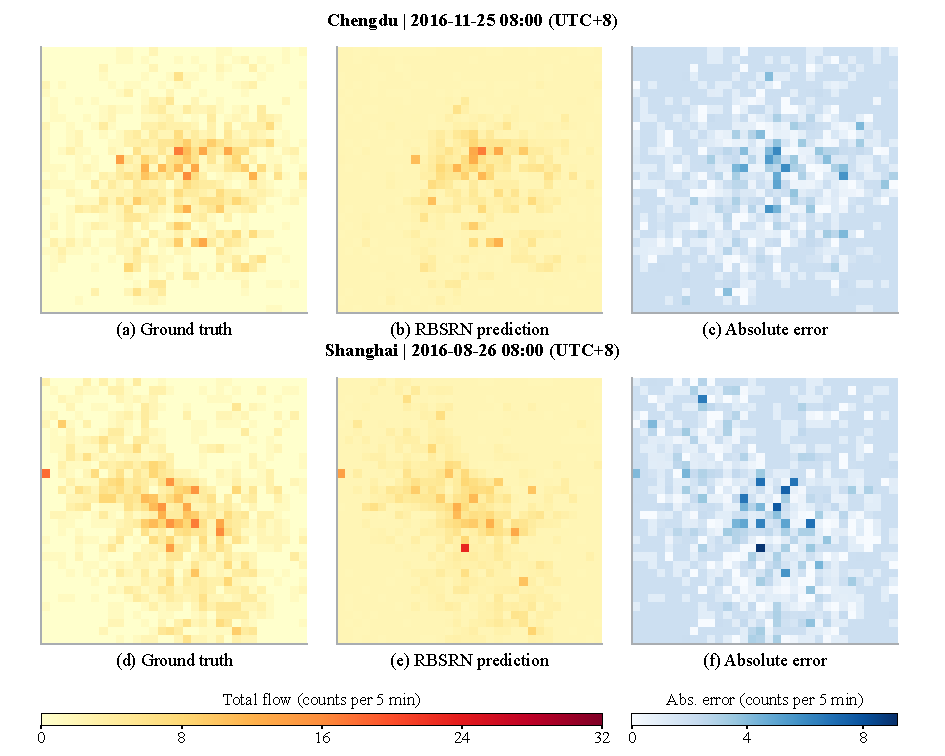
\includegraphics[width=\linewidth]{figures/spatial-fixed-morning.pdf}
  \caption{Example spatial predictions of total flow at H6 (08:00). The top and bottom rows show Chengdu and Shanghai, respectively. The columns show observations, predictions, and absolute errors.}
  \label{fig:rbsrn-spatial-h6}
\end{figure}
\FloatBarrier

% Scenario performance and analyses of the two residual pathways are included in 5.2.
% !TeX root = ../main.tex
% !TeX encoding = UTF-8

\subsubsection{Prediction Performance across Levels of Deviation from Routine Patterns}\label{sec:scenario-performance}\label{sec:exp-scenarios}

All-grid spatial statistics describe flow distribution at a given time. To examine prediction error under deviations from routine levels, we grouped observations by window, grid cell, and channel. At positions with positive H6 target flow, RBSRN was compared with 16 baselines. Chengdu scenario analysis and the subsequent residual diagnostics use a dedicated diagnostic checkpoint, whose full-test-set H6 MAE is 0.709952 for inflow and 0.709944 for outflow. The main Chengdu tables use the comparison checkpoint. Shanghai scenario analysis and residual diagnostics use the epoch-115 checkpoint reported in the main tables.

The routine-flow reference is the median training flow for the same grid cell, channel, 5-minute slot, and weekday/weekend type. We used deduplicated training-history timestamps that passed the quality checks. If a slot had fewer than four observations for one day type, the two types were pooled; if it had none, we used the grid-cell and channel median. We divided each observation's difference from its reference by a robust scale to obtain the standardized residual \(r_k\). The scale is the training residual median absolute deviation multiplied by 1.4826, with a lower bound of 1 count. The input-window deviation score is \(D=\frac{1}{12}\sum_{k=1}^{12}|r_k|\). For each city and channel, we pooled grid cells from training windows whose 12 historical steps passed the quality checks. The 50th, 80th, and 95th percentiles of \(D\) define four groups (Table~\ref{tab:scenario-group-thresholds}); boundary values enter the lower group.

\input{tables/scenario-group-thresholds}

\begin{figure}[!htbp]
  \centering
  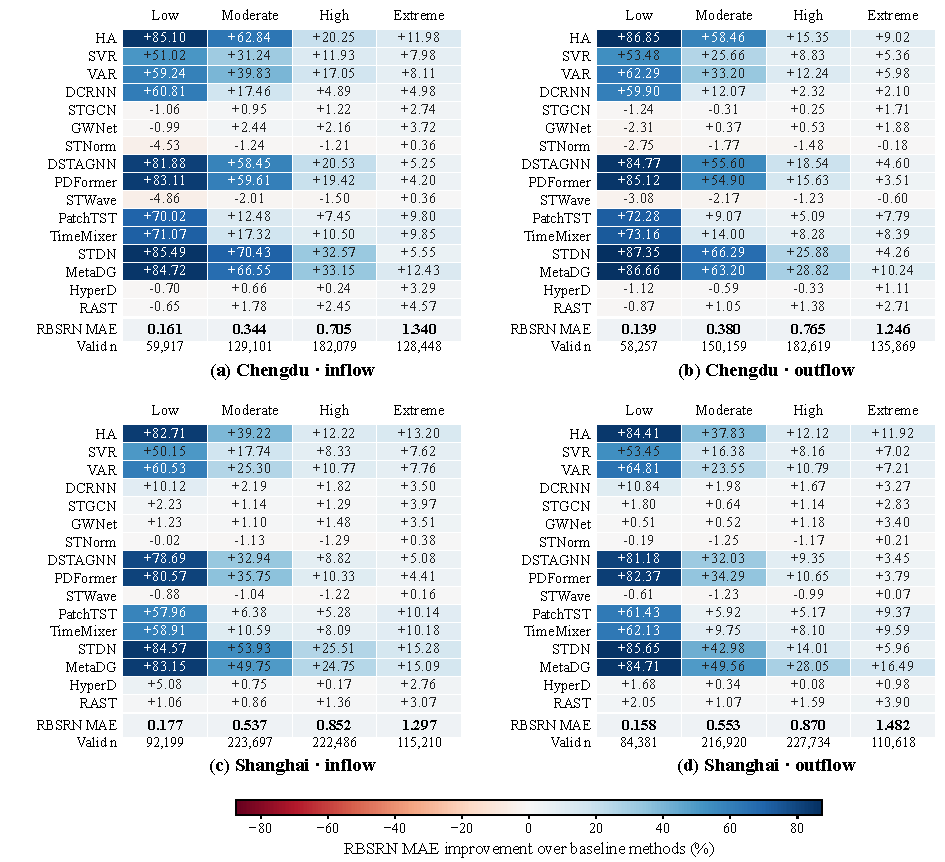
\includegraphics[width=\linewidth]{figures/scenarios/performance_h6_paper.pdf}
  \caption{RBSRN relative MAE at H6 across deviation groups.}
  \label{fig:scenario-performance}
\end{figure}

Figure~\ref{fig:scenario-performance} compares methods within each group; positive values indicate an MAE reduction relative to the corresponding baseline. In the Extreme group, RBSRN had the lowest MAE for Chengdu inflow, Shanghai inflow, and Shanghai outflow, with reductions of 0.36\%, 0.16\%, and 0.07\% relative to STWave. For Chengdu outflow, RBSRN ranked third, with MAE 0.60\% above STWave. STWave and STNorm had lower errors than RBSRN in the Moderate and High groups on all four tasks.

Absolute MAE increased with deviation level on all four tasks. Extreme-group MAE was 7.33--9.37 times the Low-group value. For Chengdu inflow, MAE increased from 0.161 to 1.340 while mean positive-target flow increased from 1.160 to 3.637 counts per 5 min, so the group differences reflect both deviation level and flow magnitude.

\subsubsection{Effects of SERR Residual Corrections across Recent-Change Scenarios}\label{sec:scenario-serr}

Within the high-deviation subset combining High and Extreme observations (\(D>D_{80}\)), recent-change intensity is defined by successive differences in historical standardized residuals:
\begin{equation}
  U=\frac{1}{11}\sum_{k=2}^{12}|r_k-r_{k-1}|.
  \label{eq:scenario-recent-change}
\end{equation}
The 75th percentile of \(U\) among high-deviation training samples separates Slow and Rapid groups; values above the threshold enter Rapid.

We examined each residual correction with a fixed-model residual-removal diagnostic. Model parameters, gates, and all other outputs were held fixed while one specified correction was subtracted from the final prediction:
\begin{equation}
  \Delta\mathrm{MAE}_{e}
  =\mathrm{MAE}(\widehat Y-C_e)-\mathrm{MAE}(\widehat Y),
  \label{eq:scenario-residual-removal}
\end{equation}
Here, \(C_e\) is the signed correction added to the prediction, including the original gating weight, learnable strength coefficient, and inverse-standardization scale. Removing the SERR self-evolution expert subtracts its weighted difference from the base prediction; removing the directed time-lagged expert subtracts its weighted correction; removing BCMS subtracts the full cross-region correction. Gating weights retain their original values and are not renormalized. A positive difference means that the correction reduced group-average MAE. Because the loss is nonlinear, differences for separate corrections are not additive. This diagnostic complements the independently retrained ablations in Section~\ref{sec:exp-ablation}: it measures sensitivity of one fixed model, whereas the ablations compare retrained configurations.

In Figure~\ref{fig:scenario-serr}, all 16 removal differences across the eight city--channel--change groups were positive. The self-evolution correction benefit in Rapid was 1.15--2.82 times the Slow-group benefit, whereas the directed time-lagged correction was smaller. Its Rapid-group benefit was higher than its Slow-group benefit in Chengdu and lower in Shanghai.

\begin{figure}[!htbp]
  \centering
  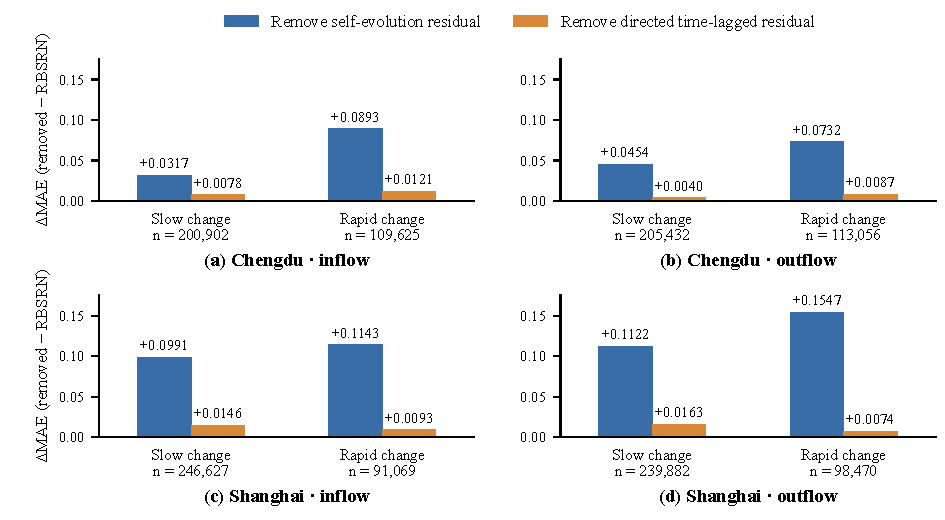
\includegraphics[width=0.92\linewidth]{figures/scenarios/serr_sensitivity_h6_paper.pdf}
\caption{H6 SERR residual-removal sensitivity by recent-change group.}
  \label{fig:scenario-serr}
\end{figure}

\subsubsection{Effects of BCMS Residual Corrections across Background Discrepancies and Forecast Horizons}\label{sec:scenario-bcms}

We measured source--target background similarity with a history-derived discrepancy proxy. Let \(\mathcal C_i\) denote the valid fixed candidate-source set for target cell \(i\), and let \(\bar r_i\) be its mean standardized residual over the 12 historical steps. For each channel, define
\begin{equation}
  B_i=\frac{1}{|\mathcal C_i|}\sum_{j\in\mathcal C_i}|\bar r_i-\bar r_j|.
  \label{eq:scenario-background-difference}
\end{equation}
The candidate set follows the model's fixed support. \(B_i\) describes discrepancy in the observed history and is separate from the low-frequency representation learned by BCMS. Tertile thresholds estimated from high-deviation training samples define Low, Medium, and High discrepancy groups (Table~\ref{tab:scenario-group-thresholds}). We removed the full BCMS correction at H1--H12 using Eq.~\eqref{eq:scenario-residual-removal}. Both figures report MAE changes in \(10^{-3}\) counts per 5 min; each cell is \(1000\times\Delta\mathrm{MAE}\).

Figure~\ref{fig:scenario-bcms} shows a consistent ordering across city, channel, and horizon: the mean benefit was largest in the Low group, followed by Medium and High. Of 144 background-group--horizon cells, 143 were positive; the only negative value was approximately \(-4.8\times10^{-6}\) for Chengdu outflow in the High group at H5. Benefits varied across horizons without a monotonic trend.

\begin{figure}[!htbp]
  \centering
  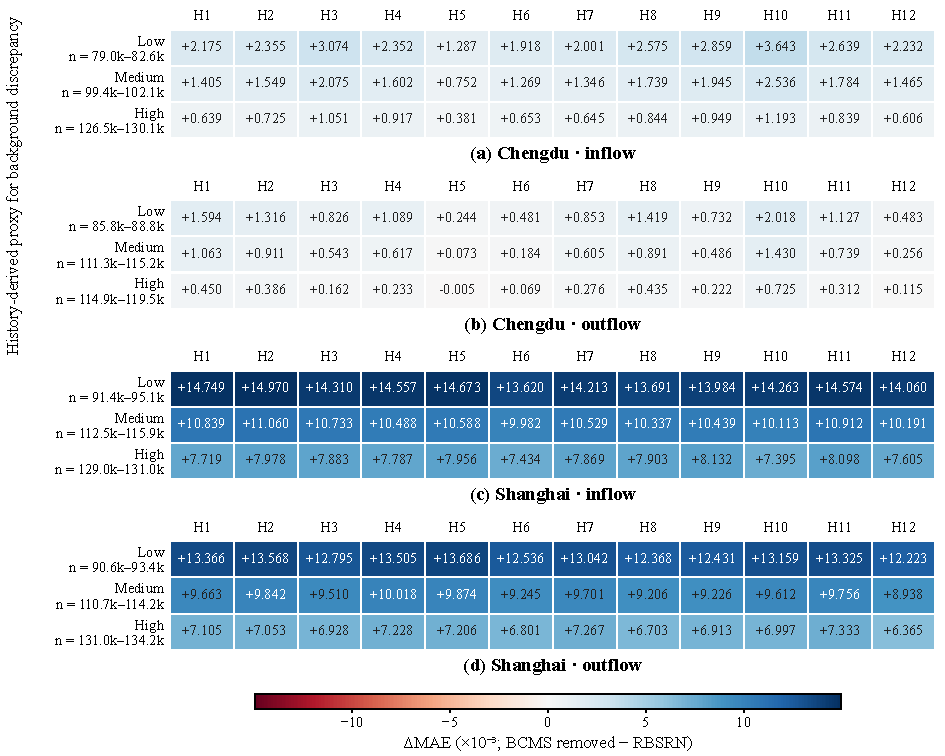
\includegraphics[width=0.92\linewidth]{figures/scenarios/bcms_sensitivity_horizons_paper.pdf}
\caption{BCMS residual-removal sensitivity in high-deviation scenarios.}
  \label{fig:scenario-bcms}
\end{figure}

Figure~\ref{fig:scenario-bcms-all} extends the analysis to the full test set with the same thresholds fitted from high-deviation training histories. All 144 removal differences were positive and exceeded the corresponding high-deviation values. The Low--Medium--High ordering persisted. For Shanghai inflow at H6, full-test differences were 0.025547, 0.015634, and 0.009873, compared with 0.013620, 0.009982, and 0.007434 in the high-deviation subset. The full-test analysis therefore shows that the average BCMS benefit extends beyond high-deviation samples.

\begin{figure}[!htbp]
  \centering
  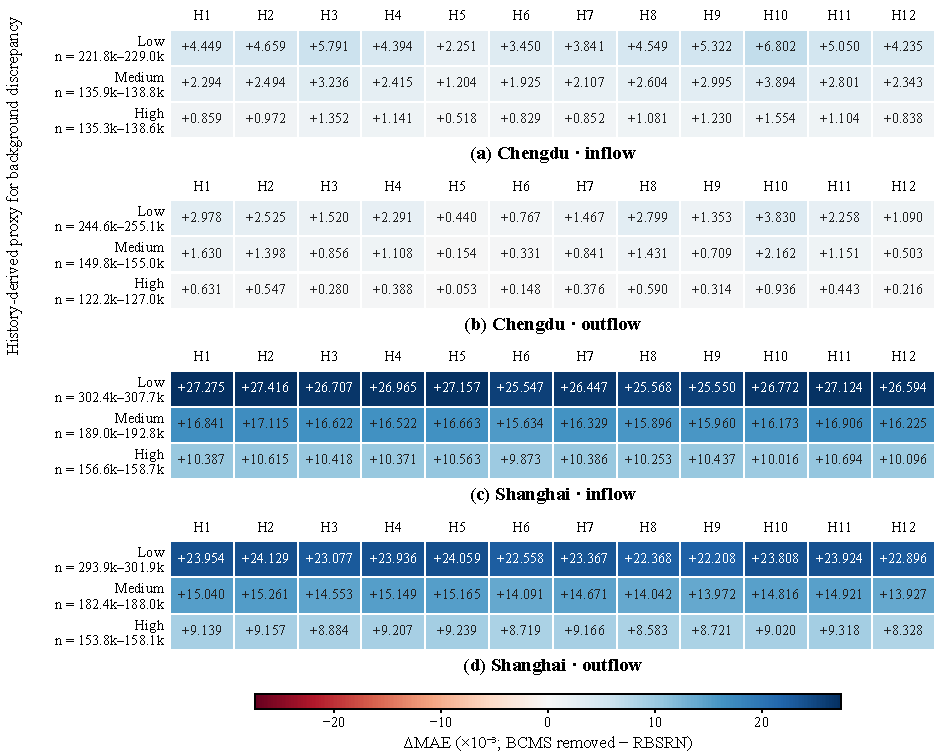
\includegraphics[width=0.92\linewidth]{figures/scenarios/bcms_sensitivity_horizons_all_test_paper.pdf}
\caption{BCMS residual-removal sensitivity across the full test set.}
  \label{fig:scenario-bcms-all}
\end{figure}



% !TeX root = ../main.tex
% !TeX encoding = UTF-8
\subsection{Ablation Study}\label{sec:exp-ablation}

We evaluated the three residual pathways with Chengdu ablations. A1 removes the self-evolution expert, A2 removes the directed time-lagged expert, and A3 removes BCMS. Each variant was retrained for up to 200 epochs with an early-stopping patience of 20 epochs. In A1 and A2, the remaining expert weights were renormalized after setting the removed weight to zero. Testing used the positive-target mask and AVG12 aggregation defined in Section~\ref{sec:exp-baselines-metrics}. Joint MAE and RMSE are the equal-weight averages of the inflow and outflow AVG12 values.

% !TeX root = ../main.tex
\begin{table}[!htbp]
  \centering
  \caption{Chengdu ablation results (AVG12)}
  \label{tab:serr-expert-ablation}
  \begingroup
  \linespread{1}\fontsize{9}{11}\selectfont
  \setlength{\tabcolsep}{3pt}
  \renewcommand{\arraystretch}{1.08}
  \begin{tabular*}{\linewidth}{@{\extracolsep{\fill}}lrrrrrr@{}}
    \toprule
    Model configuration & \shortstack{Inflow\\MAE} & \shortstack{Inflow\\RMSE} & \shortstack{Outflow\\MAE} & \shortstack{Outflow\\RMSE} & \shortstack{Joint\\MAE} & \shortstack{Joint\\RMSE} \\
    \midrule
    RBSRN & \ablationpolished{\textbf{0.7084}} & \ablationpolished{\textbf{1.2935}} & \ablationpolished{\textbf{0.7087}} & \ablationpolished{\textbf{1.2235}} & \ablationpolished{\textbf{0.7085}} & \ablationpolished{\textbf{1.2585}} \\
    w/o Self-evolution expert (A1) & \ablationpolished{0.7129} & \ablationpolished{1.3037} & \ablationpolished{0.7121} & \ablationpolished{1.2270} & \ablationpolished{0.7125} & \ablationpolished{1.2653} \\
    w/o Directed time-lagged expert (A2) & \ablationpolished{0.7105} & \ablationpolished{1.3048} & \ablationpolished{0.7099} & \ablationpolished{1.2264} & \ablationpolished{0.7102} & \ablationpolished{1.2656} \\
    w/o BCMS (A3) & \ablationpolished{0.7109} & \ablationpolished{1.3014} & \ablationpolished{0.7102} & \ablationpolished{1.2276} & \ablationpolished{0.7105} & \ablationpolished{1.2645} \\
    \bottomrule
  \end{tabular*}
  \endgroup
\end{table}

\FloatBarrier

Table~\ref{tab:serr-expert-ablation} shows that the full RBSRN had the lowest error on all six metrics. Removing any branch increased MAE and RMSE for both flows. Removing the self-evolution expert increased joint MAE by 0.56\%, the largest increase among the variants. Removing the directed time-lagged expert increased joint RMSE by 0.56\%, compared with 0.54\% for removing self-evolution. The two experts therefore contribute through different error measures, with self-evolution having the larger effect on joint MAE.

Removing BCMS increased joint MAE and RMSE by 0.28\% and 0.48\%, respectively, with higher errors for both flows. The full model performed best when self-evolution, directed time-lagged association, and background-conditioned message selection were combined.
\FloatBarrier


% !TeX root = ../main.tex
% !TeX encoding = UTF-8
% !TeX spellcheck = none
\subsection{Hyperparameter Sensitivity Analysis}\label{sec:exp-hyperparameters}

\hpupdated{We conducted one-factor-at-a-time validation experiments on Chengdu to examine how SERR gating capacity, BCMS representation capacity, and the initial values of two residual pathways affect prediction error. The SERR gating hidden dimension and the BCMS internal representation dimension each took values in \(\{8,16,32,64,128\}\). Both \(\alpha_0\) and \(\beta_0\) took values in \(\{0,0.001,0.01,0.05,0.1\}\). They specify the initial values of the learnable residual parameters defined in Sections~\ref{sec:serr} and~\ref{sec:bcms}, respectively, and these parameters continue to update during training. The reference configuration was \((32,32,0,0)\), as used in the main comparison experiments. We changed one parameter at a time while keeping all other settings fixed. \editorialupdated{Bold tick labels indicate the reference configuration, and the minimum within each group was determined from unrounded results.} Training, checkpoint selection, and validation aggregation followed Sections~\ref{sec:exp-implementation} and~\ref{sec:exp-datasets}.}

\hpupdated{We first constructed the model with the reference configuration and replaced the gating or BCMS module only when its dimension differed from 32. Residual initial values were assigned directly to the learnable parameters. Neither training nor validation used additional splitting into microbatches.}

\hpupdated{All four parameters produced only small changes in joint validation error within the tested ranges (Figure~\ref{fig:hyperparameter-joint}). We calculated each group's relative range as the difference between its maximum and minimum errors divided by the error of the reference configuration. Across the four groups, this range was below 0.15\% for joint MAE and below 0.35\% for joint RMSE.}

\begin{figure}[!htbp]
  \centering
  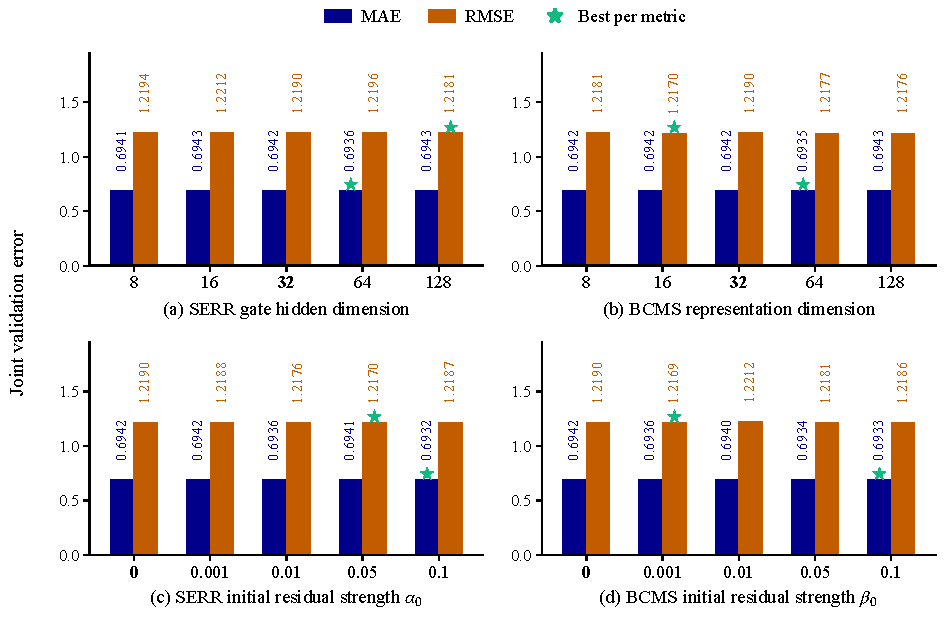
\includegraphics[width=\linewidth]{figures/hyperparameter-joint.pdf}
  \caption{\editorialupdated{Hyperparameter sensitivity of joint validation metrics on the Chengdu dataset.}}
  \label{fig:hyperparameter-joint}
\end{figure}

\hpupdated{Increasing the hidden dimension did not consistently reduce error, and the lowest joint MAE and RMSE occurred at different dimensions. The best positive initial values of the residual parameters provided only small improvements over zero initialization. The two metrics likewise did not share a single optimal initial value.}

\hpupdated{Figure~\ref{fig:hyperparameter-flow} presents the complete results for each flow channel. The small changes in joint error also included different responses across channels. For the SERR gating dimension, inflow MAE was lowest at 64, whereas outflow MAE was lowest at 8. Thus, the two flow channels responded differently to gating capacity.}

\begin{figure}[!htbp]
  \centering
  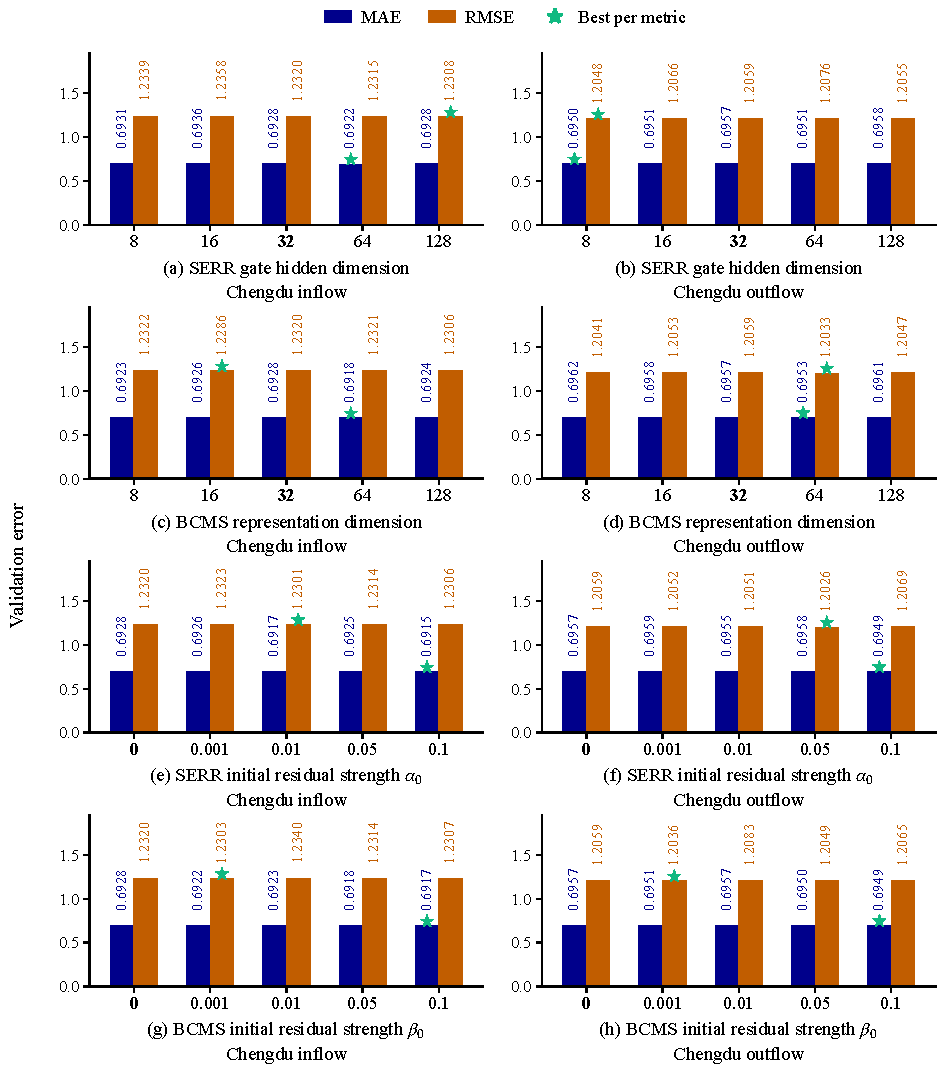
\includegraphics[width=\linewidth]{figures/hyperparameter-flow.pdf}
  \caption{\editorialupdated{Hyperparameter sensitivity for inflow and outflow on the Chengdu dataset.}}
  \label{fig:hyperparameter-flow}
\end{figure}
\FloatBarrier


% !TeX root = ../main.tex
\subsection{Model Size and Inference Efficiency}\label{sec:exp-efficiency}

With both the gating and BCMS dimensions set to 32, RBSRN contains approximately 7.071 million trainable parameters. We evaluated inference efficiency using the Chengdu checkpoint from the main comparison experiments. Each batch-size setting used a single NVIDIA A100-SXM4-40GB GPU with FP32 tensors; the remaining computing environment is described in Section~\ref{sec:exp-implementation}. Each window supplies 12 historical flow steps and jointly produces inflow and outflow forecasts for 1,024 nodes over the next 12 steps.

For batch size 1, we used compiled BCMS operators and CUDA Graph, with 20 warm-up iterations followed by 100 timed iterations. For batch size 64, we used compiled BCMS operators, with 10 warm-up iterations followed by 30 timed iterations. CUDA synchronization was performed before and after each measurement. We report the median and 95th percentile (P95), which describe typical execution time and tail latency within these measurements, respectively.

Forward-only timing includes model computation on GPU-resident inputs and excludes copying new inputs. End-to-end timing covers memory-resident data access, wavelet decomposition, normalization, state-evidence construction, CPU/GPU transfers, model inference, inverse standardization, and returning results to the CPU. It also includes input updates before CUDA Graph replay. Both measurements exclude startup preparation, offline graph construction, and cold disk reads. Startup preparation comprises initialization, compilation, graph capture, and warm-up.

\begin{table}[!htbp]
	\centering
	\small
	\caption{RBSRN inference time on the Chengdu dataset}
	\label{tab:inference-latency}
	\begin{tabular*}{\linewidth}{@{\extracolsep{\fill}}lcrrrr@{}}
		\toprule
		Inference setting & Batch size
		& \multicolumn{2}{c}{\shortstack{Forward only\\ms/batch}}
		& \multicolumn{2}{c}{\shortstack{End to end\\ms/batch}} \\
		\cmidrule(lr){3-4}\cmidrule(lr){5-6}
		& & Median & P95 & Median & P95 \\
		\midrule
		\shortstack[l]{Single-window\\forecasting} & 1  & 15.907   & 15.930   & 19.228   & 19.507 \\
		Batch forecasting   & 64 & 1138.819 & 1310.517 & 1280.394 & 1464.308 \\
		\bottomrule
	\end{tabular*}
\end{table}

Table~\ref{tab:inference-latency} reports median forward-only and end-to-end latencies of 15.907\,ms and 19.228\,ms for single-window forecasting, with an end-to-end P95 of 19.507\,ms. In this test environment, the measured computation time fit within a 5-minute update cycle. At batch size 64, the median end-to-end time was 1,280.394\,ms/batch, and the amortized forward-only time was 17.794\,ms/window. The batch-size-1 measurements characterize the response time of an individual request.

The inference configurations above used the same model checkpoint. We compared each against the reference implementation at the same batch size. At batch size 64, checking all 1,723 test windows yielded a maximum absolute prediction difference of \(7.63\times10^{-6}\). Batch size 1 passed a sampled check against the reference at the same batch size. Aggregate forecasting metrics were similar across the two batch sizes, although individual predictions were not identical. All main accuracy results were evaluated at batch size 64.

\FloatBarrier


\FloatBarrier
% !TeX root = ../main.tex
% !TeX encoding = UTF-8
% !TeX spellcheck = none

\begingroup
\conclusionrevisionstyle
\section{Conclusion}\label{sec:conclusion}

We present RBSRN, a role-aware and background-conditioned spatiotemporal residual network for short-term, multi-step regional inflow and outflow forecasting. It refines a shared base prediction through state-conditioned expert correction and background-conditioned historical message selection. In experiments over forecast horizons of 5--60 minutes in Chengdu and Shanghai, we compared RBSRN with 13 baseline methods under positive-target evaluation. RBSRN achieved the lowest AVG12 MAE and RMSE across all four city--channel tasks. Its MAE was 0.43\%--2.00\% lower than that of the strongest baseline method for each task.

Ablation experiments and fixed-model diagnostics supported complementary roles for SERR and BCMS. In H6 diagnostics on high-deviation samples, self-evolution correction provided larger absolute MAE benefits for rapidly changing histories than for slowly changing histories. The effects of directed time-lagged correction varied across cities. BCMS provided larger mean benefits when the history-derived proxy for background discrepancy was smaller, and these benefits extended beyond high-deviation scenarios. RBSRN did not outperform the strongest baseline methods in every deviation group, indicating that its advantages depended on the traffic state.

The empirical evaluation is limited to one month of data from each city. Future work should evaluate temporal generalization across months and seasons, assess the benefits and computational costs of dynamically updating candidate relations, and compare all methods under both positive-target and all-grid evaluation. These extensions would clarify the robustness and practical applicability of the proposed correction mechanisms.
\endgroup


\FloatBarrier
% !TeX root = main.tex
% !TeX spellcheck = none
% 2026-11-06: 41 cited works, reverified and ordered by first appearance in main.tex.
% Stable citation keys identify papers; they are not display numbers.
% Field and placement audit: source/citation-order-20261106/.
\begingroup
\citationbibliographystyle
\linespread{1.05}\selectfont
\begin{thebibliography}{99}
\setlength{\itemsep}{3pt}
\bibitem{ref44}
F. Rodrigues, I. Markou, and F. C. Pereira, ``Combining time-series and textual data for taxi demand prediction in event areas: A deep learning approach,'' \emph{Inf. Fusion}, vol. 49, pp. 120--129, 2019, doi: \href{https://doi.org/10.1016/j.inffus.2018.07.007}{10.1016/j.inffus.2018.07.007}.

\bibitem{ref36}
J. Sun, J. Zhang, Q. Li, X. Yi, Y. Liang, and Y. Zheng, ``Predicting citywide crowd flows in irregular regions using multi-view graph convolutional networks,'' \emph{IEEE Trans. Knowl. Data Eng.}, vol. 34, no. 5, pp. 2348--2359, 2022, doi: \href{https://doi.org/10.1109/TKDE.2020.3008774}{10.1109/TKDE.2020.3008774}.

\bibitem{ref27}
E. Kontou, V. Garikapati, and Y. Hou, ``Reducing ridesourcing empty vehicle travel with future travel demand prediction,'' \emph{Transp. Res. C, Emerg. Technol.}, vol. 121, Art. no. 102826, 2020, doi: \href{https://doi.org/10.1016/j.trc.2020.102826}{10.1016/j.trc.2020.102826}.

\bibitem{ref43}
J. Ke, H. Zheng, H. Yang, and X. Chen, ``Short-term forecasting of passenger demand under on-demand ride services: A spatio-temporal deep learning approach,'' \emph{Transp. Res. C, Emerg. Technol.}, vol. 85, pp. 591--608, 2017, doi: \href{https://doi.org/10.1016/j.trc.2017.10.016}{10.1016/j.trc.2017.10.016}.

\bibitem{ref42}
A. Essien, I. Petrounias, P. Sampaio, and S. Sampaio, ``A deep-learning model for urban traffic flow prediction with traffic events mined from Twitter,'' \emph{World Wide Web}, vol. 24, no. 4, pp. 1345--1368, 2021, doi: \href{https://doi.org/10.1007/s11280-020-00800-3}{10.1007/s11280-020-00800-3}.

\bibitem{ref14}
J. Zhang, Y. Zheng, and D. Qi, ``Deep spatio-temporal residual networks for citywide crowd flows prediction,'' in \emph{Proc. AAAI Conf. Artif. Intell.}, vol. 31, no. 1, 2017, pp. 1655--1661, doi: \href{https://doi.org/10.1609/aaai.v31i1.10735}{10.1609/aaai.v31i1.10735}.

\bibitem{ref01}
Y. Li, R. Yu, C. Shahabi, and Y. Liu, ``Diffusion convolutional recurrent neural network: Data-driven traffic forecasting,'' in \emph{Proc. Int. Conf. Learn. Represent. (ICLR)}, 2018.

\bibitem{ref02}
B. Yu, H. Yin, and Z. Zhu, ``Spatio-temporal graph convolutional networks: A deep learning framework for traffic forecasting,'' in \emph{Proc. 27th Int. Joint Conf. Artif. Intell. (IJCAI)}, 2018, pp. 3634--3640, doi: \href{https://doi.org/10.24963/ijcai.2018/505}{10.24963/ijcai.2018/505}.

\bibitem{ref03}
Z. Wu, S. Pan, G. Long, J. Jiang, and C. Zhang, ``Graph WaveNet for deep spatial-temporal graph modeling,'' in \emph{Proc. 28th Int. Joint Conf. Artif. Intell. (IJCAI)}, 2019, pp. 1907--1913, doi: \href{https://doi.org/10.24963/ijcai.2019/264}{10.24963/ijcai.2019/264}.

\bibitem{ref11}
Y. Fang \emph{et al.}, ``When spatio-temporal meet wavelets: Disentangled traffic forecasting via efficient spectral graph attention networks,'' in \emph{Proc. IEEE 39th Int. Conf. Data Eng. (ICDE)}, 2023, pp. 517--529, doi: \href{https://doi.org/10.1109/ICDE55515.2023.00046}{10.1109/ICDE55515.2023.00046}.

\bibitem{ref18}
Y. Xu, L. Wei, and L. Feng, ``A spatial-temporal trend-event decoupling dual-channel framework for traffic flow prediction,'' \emph{Expert Syst. Appl.}, vol. 287, Art. no. 128107, 2025, doi: \href{https://doi.org/10.1016/j.eswa.2025.128107}{10.1016/j.eswa.2025.128107}.

\bibitem{ref41}
X. Zhang \emph{et al.}, ``Traffic flow forecasting with spatial-temporal graph diffusion network,'' in \emph{Proc. AAAI Conf. Artif. Intell.}, vol. 35, no. 17, 2021, pp. 15008--15015, doi: \href{https://doi.org/10.1609/aaai.v35i17.17761}{10.1609/aaai.v35i17.17761}.

\bibitem{ref47}
Q. Long, Z. Fang, C. Fang, C. Chen, P. Wang, and Y. Zhou, ``Unveiling delay effects in traffic forecasting: A perspective from spatial-temporal delay differential equations,'' in \emph{Proc. ACM Web Conf.}, 2024, pp. 1035--1044, doi: \href{https://doi.org/10.1145/3589334.3645688}{10.1145/3589334.3645688}.

\bibitem{ref25}
Z. Shao \emph{et al.}, ``Decoupled dynamic spatial-temporal graph neural network for traffic forecasting,'' \emph{Proc. VLDB Endow.}, vol. 15, no. 11, pp. 2733--2746, 2022, doi: \href{https://doi.org/10.14778/3551793.3551827}{10.14778/3551793.3551827}.

\bibitem{ref26}
H. Lee and S. Ko, ``TESTAM: A time-enhanced spatio-temporal attention model with mixture of experts,'' in \emph{Proc. Int. Conf. Learn. Represent. (ICLR)}, 2024.

\bibitem{ref10}
J. Jiang, C. Han, W. X. Zhao, and J. Wang, ``PDFormer: Propagation delay-aware dynamic long-range Transformer for traffic flow prediction,'' in \emph{Proc. AAAI Conf. Artif. Intell.}, vol. 37, no. 4, 2023, pp. 4365--4373, doi: \href{https://doi.org/10.1609/aaai.v37i4.25556}{10.1609/aaai.v37i4.25556}.

\bibitem{ref29}
R. Jiang \emph{et al.}, ``DL-Traff: Survey and benchmark of deep learning models for urban traffic prediction,'' in \emph{Proc. 30th ACM Int. Conf. Inf. Knowl. Manage. (CIKM)}, 2021, pp. 4515--4525, doi: \href{https://doi.org/10.1145/3459637.3482000}{10.1145/3459637.3482000}.

\bibitem{ref28}
Z. Shao, Z. Zhang, F. Wang, W. Wei, and Y. Xu, ``Spatial-temporal identity: A simple yet effective baseline for multivariate time series forecasting,'' in \emph{Proc. 31st ACM Int. Conf. Inf. Knowl. Manage. (CIKM)}, 2022, pp. 4454--4458, doi: \href{https://doi.org/10.1145/3511808.3557702}{10.1145/3511808.3557702}.

\bibitem{ref04}
S. Guo, Y. Lin, N. Feng, C. Song, and H. Wan, ``Attention based spatial-temporal graph convolutional networks for traffic flow forecasting,'' in \emph{Proc. AAAI Conf. Artif. Intell.}, vol. 33, no. 1, 2019, pp. 922--929, doi: \href{https://doi.org/10.1609/aaai.v33i01.3301922}{10.1609/aaai.v33i01.3301922}.

\bibitem{ref05}
C. Zheng, X. Fan, C. Wang, and J. Qi, ``GMAN: A graph multi-attention network for traffic prediction,'' in \emph{Proc. AAAI Conf. Artif. Intell.}, vol. 34, no. 1, 2020, pp. 1234--1241, doi: \href{https://doi.org/10.1609/aaai.v34i01.5477}{10.1609/aaai.v34i01.5477}.

\bibitem{ref06}
Z. Wu, S. Pan, G. Long, J. Jiang, X. Chang, and C. Zhang, ``Connecting the dots: Multivariate time series forecasting with graph neural networks,'' in \emph{Proc. 26th ACM SIGKDD Int. Conf. Knowl. Discov. Data Min. (KDD)}, 2020, pp. 753--763, doi: \href{https://doi.org/10.1145/3394486.3403118}{10.1145/3394486.3403118}.

\bibitem{ref07}
L. Bai, L. Yao, C. Li, X. Wang, and C. Wang, ``Adaptive graph convolutional recurrent network for traffic forecasting,'' in \emph{Adv. Neural Inf. Process. Syst. (NeurIPS)}, vol. 33, 2020, pp. 17804--17815.

\bibitem{ref08}
C. Song, Y. Lin, S. Guo, and H. Wan, ``Spatial-temporal synchronous graph convolutional networks: A new framework for spatial-temporal network data forecasting,'' in \emph{Proc. AAAI Conf. Artif. Intell.}, vol. 34, no. 1, 2020, pp. 914--921, doi: \href{https://doi.org/10.1609/aaai.v34i01.5438}{10.1609/aaai.v34i01.5438}.

\bibitem{ref09}
M. Li and Z. Zhu, ``Spatial-temporal fusion graph neural networks for traffic flow forecasting,'' in \emph{Proc. AAAI Conf. Artif. Intell.}, vol. 35, no. 5, 2021, pp. 4189--4196, doi: \href{https://doi.org/10.1609/aaai.v35i5.16542}{10.1609/aaai.v35i5.16542}.

\bibitem{ref37}
X. Su, F. Liu, Y. Chang, E. Tanin, M. Sarvi, and J. Qi, ``DualCast: A model to disentangle aperiodic events from traffic series,'' in \emph{Proc. 34th Int. Joint Conf. Artif. Intell. (IJCAI)}, 2025, pp. 3290--3298, doi: \href{https://doi.org/10.24963/ijcai.2025/366}{10.24963/ijcai.2025/366}.

\bibitem{ref22}
M. Shao, Z. Zhang, Y. Wang, Y. Dai, X. Shen, and X. Wang, ``HyperD: Hybrid periodicity decoupling framework for traffic forecasting,'' in \emph{Proc. AAAI Conf. Artif. Intell.}, vol. 40, no. 18, 2026, pp. 15689--15697, doi: \href{https://doi.org/10.1609/aaai.v40i18.38599}{10.1609/aaai.v40i18.38599}.

\bibitem{ref30}
J. Ji \emph{et al.}, ``Spatio-temporal self-supervised learning for traffic flow prediction,'' in \emph{Proc. AAAI Conf. Artif. Intell.}, vol. 37, no. 4, 2023, pp. 4356--4364, doi: \href{https://doi.org/10.1609/aaai.v37i4.25555}{10.1609/aaai.v37i4.25555}.

\bibitem{ref40}
M. Li, P. Tong, M. Li, Z. Jin, J. Huang, and X.-S. Hua, ``Traffic flow prediction with vehicle trajectories,'' in \emph{Proc. AAAI Conf. Artif. Intell.}, vol. 35, no. 1, 2021, pp. 294--302, doi: \href{https://doi.org/10.1609/aaai.v35i1.16104}{10.1609/aaai.v35i1.16104}.

\bibitem{ref39}
H. Yao, X. Tang, H. Wei, G. Zheng, and Z. Li, ``Revisiting spatial-temporal similarity: A deep learning framework for traffic prediction,'' in \emph{Proc. AAAI Conf. Artif. Intell.}, vol. 33, no. 1, 2019, pp. 5668--5675, doi: \href{https://doi.org/10.1609/aaai.v33i01.33015668}{10.1609/aaai.v33i01.33015668}.

\bibitem{ref31}
R. Jiang \emph{et al.}, ``Spatio-temporal meta-graph learning for traffic forecasting,'' in \emph{Proc. AAAI Conf. Artif. Intell.}, vol. 37, no. 7, 2023, pp. 8078--8086, doi: \href{https://doi.org/10.1609/aaai.v37i7.25976}{10.1609/aaai.v37i7.25976}.

\bibitem{ref23}
W. Ruan, X. Dang, Z. Zhou, S. Lyu, and Y. Liang, ``A retrieval augmented spatio-temporal framework for traffic prediction,'' in \emph{Proc. AAAI Conf. Artif. Intell.}, vol. 40, no. 46, 2026, pp. 39163--39172, doi: \href{https://doi.org/10.1609/aaai.v40i46.41264}{10.1609/aaai.v40i46.41264}.

\bibitem{ref46}
Z. Pan \emph{et al.}, ``Spatio-temporal meta learning for urban traffic prediction,'' \emph{IEEE Trans. Knowl. Data Eng.}, vol. 34, no. 3, pp. 1462--1476, 2022, doi: \href{https://doi.org/10.1109/TKDE.2020.2995855}{10.1109/TKDE.2020.2995855}.

\bibitem{ref32}
J. Ke, X. Qin, H. Yang, Z. Zheng, Z. Zhu, and J. Ye, ``Predicting origin-destination ride-sourcing demand with a spatio-temporal encoder-decoder residual multi-graph convolutional network,'' \emph{Transp. Res. C, Emerg. Technol.}, vol. 122, Art. no. 102858, 2021, doi: \href{https://doi.org/10.1016/j.trc.2020.102858}{10.1016/j.trc.2020.102858}.

\bibitem{ref45}
E. Perez, F. Strub, H. de Vries, V. Dumoulin, and A. Courville, ``FiLM: Visual reasoning with a general conditioning layer,'' in \emph{Proc. AAAI Conf. Artif. Intell.}, vol. 32, no. 1, 2018, pp. 3942--3951, doi: \href{https://doi.org/10.1609/aaai.v32i1.11671}{10.1609/aaai.v32i1.11671}.

\bibitem{ref19}
S. Lan, Y. Ma, W. Huang, W. Wang, H. Yang, and P. Li, ``DSTAGNN: Dynamic spatial-temporal aware graph neural network for traffic flow forecasting,'' in \emph{Proc. 39th Int. Conf. Mach. Learn. (ICML)}, vol. 162, 2022, pp. 11906--11917.

\bibitem{ref20}
L. Cao, B. Wang, G. Jiang, Y. Yu, and J. Dong, ``Spatiotemporal-aware trend-seasonality decomposition network for traffic flow forecasting,'' in \emph{Proc. AAAI Conf. Artif. Intell.}, vol. 39, no. 11, 2025, pp. 11463--11471, doi: \href{https://doi.org/10.1609/aaai.v39i11.33247}{10.1609/aaai.v39i11.33247}.

\bibitem{ref21}
Y. Zou, H. Yuan, Q. Yang, Z. Yuan, S. Wang, and S. Ruan, ``Meta dynamic graph for traffic flow prediction,'' in \emph{Proc. AAAI Conf. Artif. Intell.}, vol. 40, no. 19, 2026, pp. 16584--16592, doi: \href{https://doi.org/10.1609/aaai.v40i19.38699}{10.1609/aaai.v40i19.38699}.

\bibitem{ref12}
Y. Nie, N. H. Nguyen, P. Sinthong, and J. Kalagnanam, ``A time series is worth 64 words: Long-term forecasting with Transformers,'' in \emph{Proc. Int. Conf. Learn. Represent. (ICLR)}, 2023.

\bibitem{ref13}
S. Wang \emph{et al.}, ``TimeMixer: Decomposable multiscale mixing for time series forecasting,'' in \emph{Proc. Int. Conf. Learn. Represent. (ICLR)}, 2024.

\bibitem{ref24}
J. Deng, X. Chen, R. Jiang, X. Song, and I. W. Tsang, ``ST-Norm: Spatial and temporal normalization for multi-variate time series forecasting,'' in \emph{Proc. 27th ACM SIGKDD Conf. Knowl. Discov. Data Min. (KDD)}, 2021, pp. 269--278, doi: \href{https://doi.org/10.1145/3447548.3467330}{10.1145/3447548.3467330}.

\end{thebibliography}
\endgroup

\end{document}
